\section{Anhang}
\subsection{Amplitudengänge}
\subsubsection{Tiefpässe}

\begin{figure}[h]
\centering
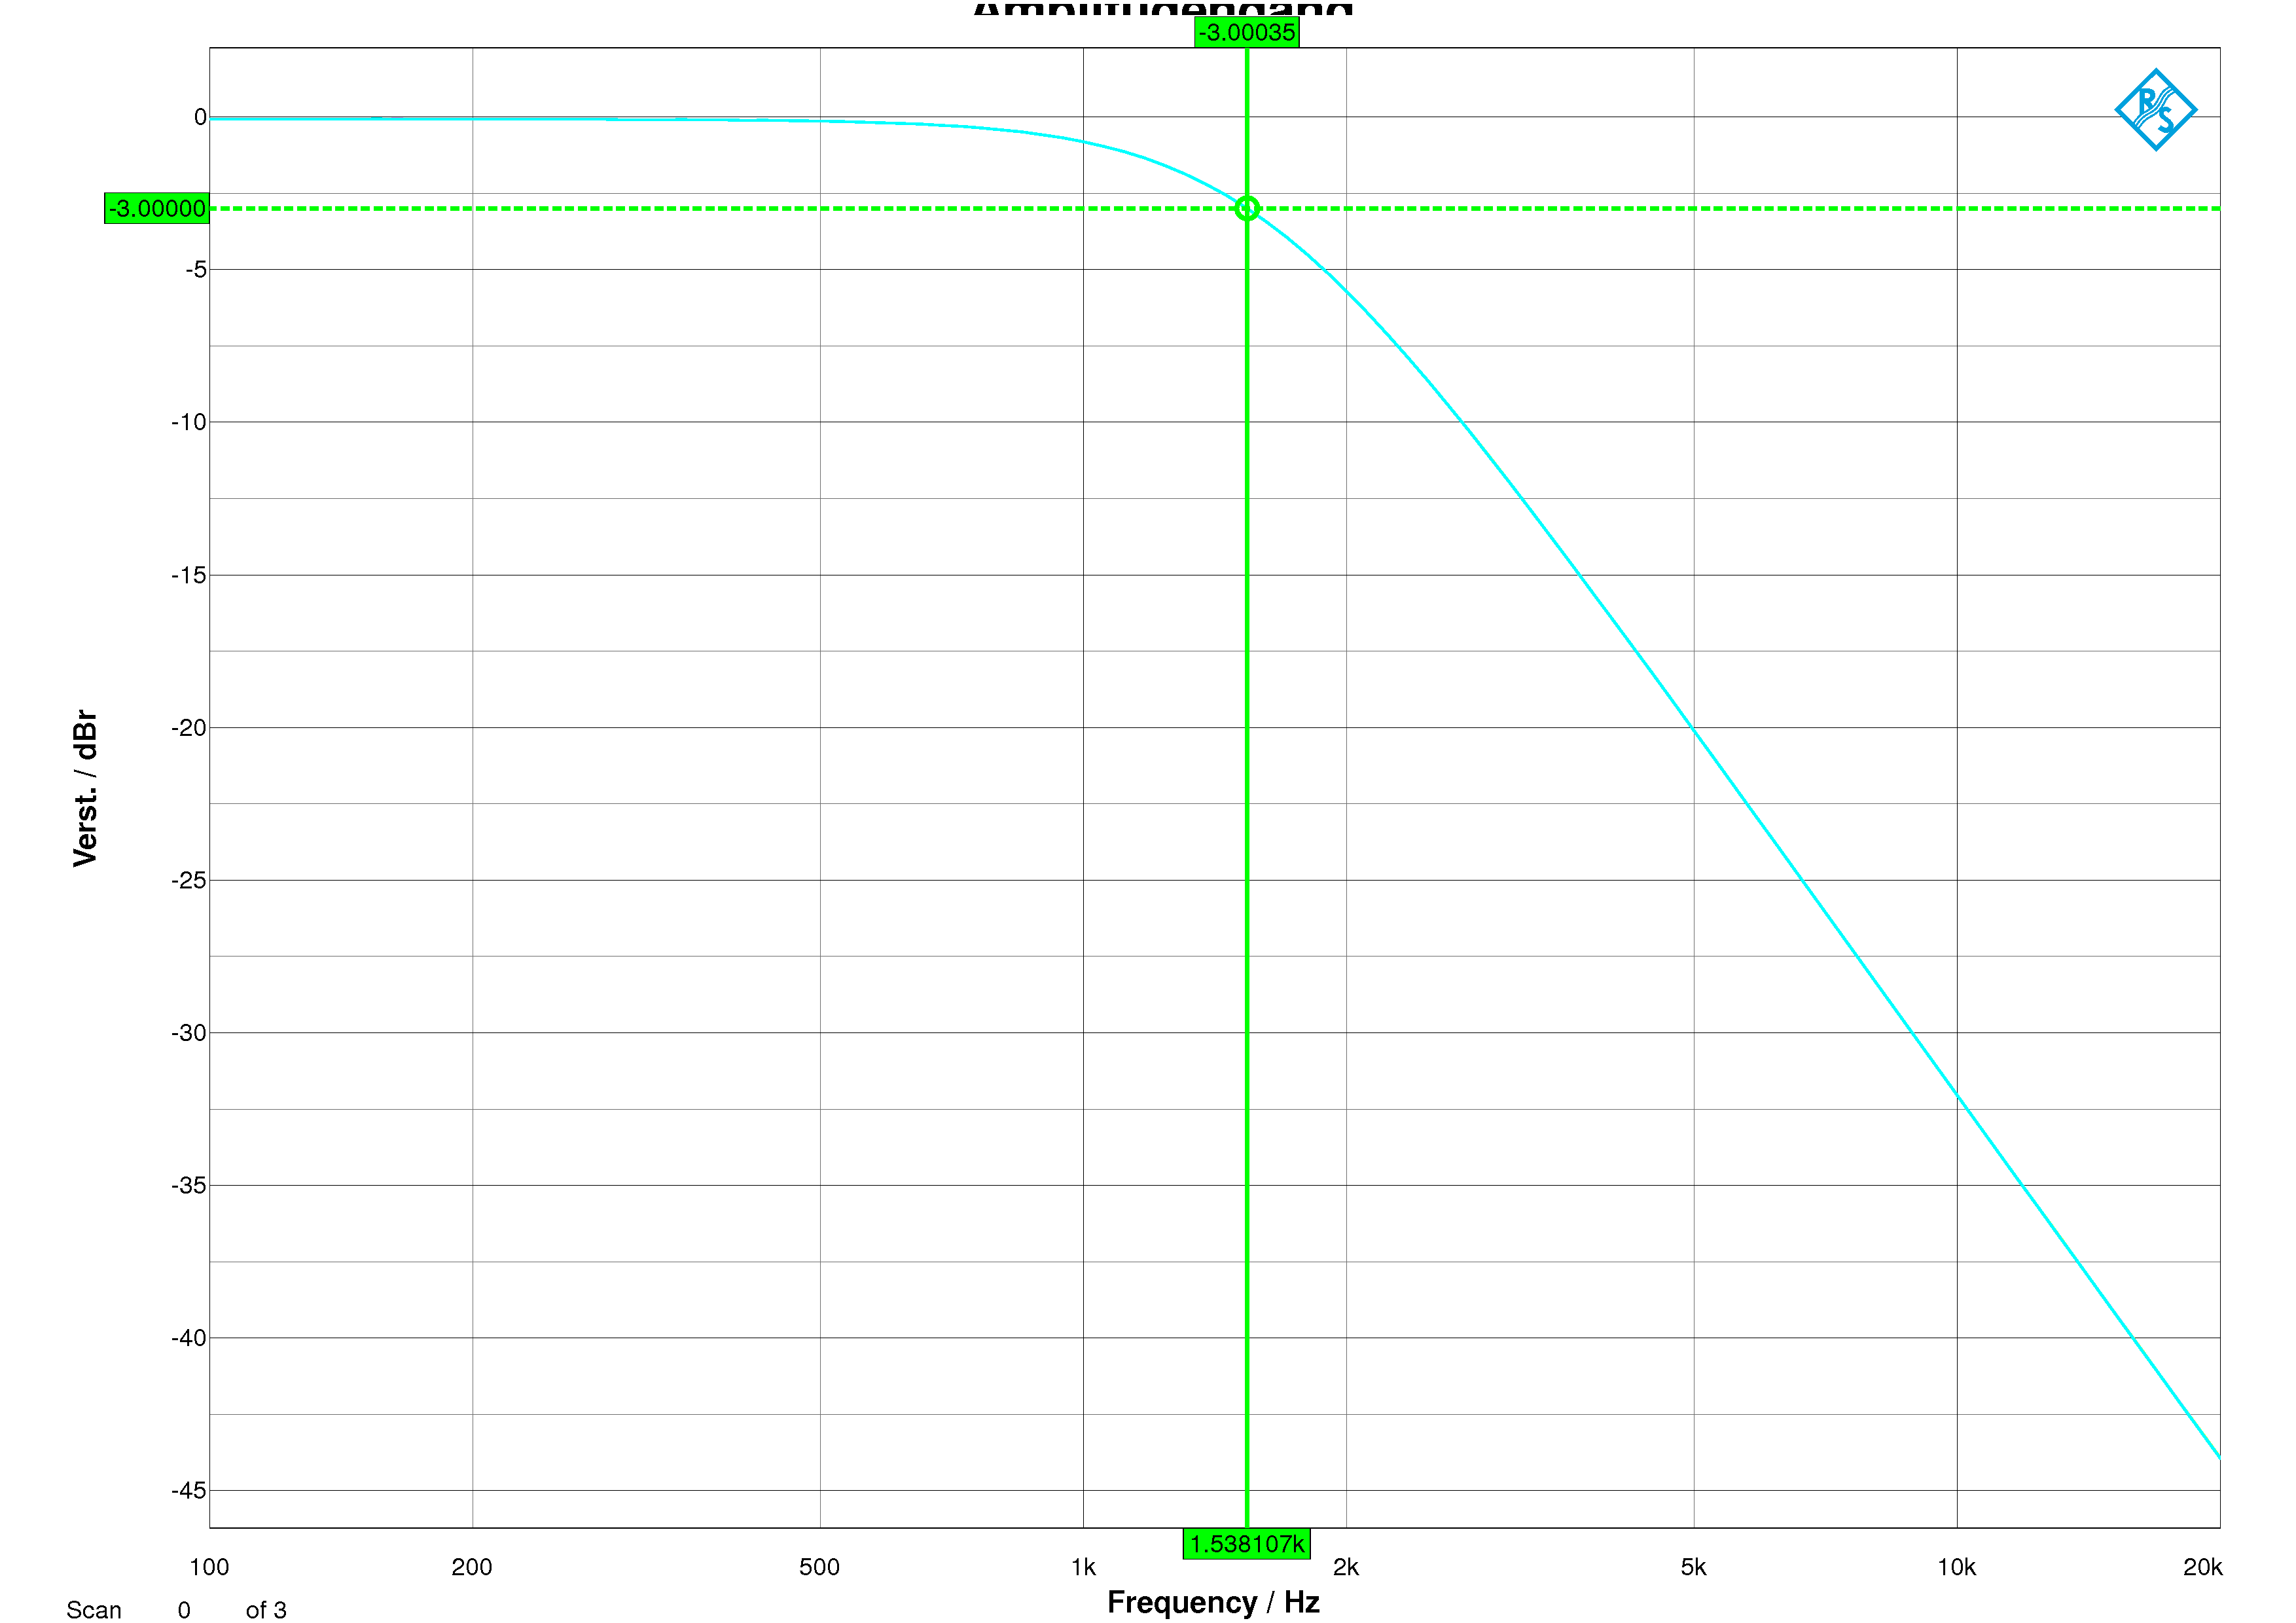
\includegraphics[width=0.60\linewidth]{Bilder/ImLabor/Amplitudengang_2_1_Butter_TP}
\caption{Amplitudengang Butterworth-Tiefpass mit Marker}
\label{fig:Amplitudengang_2_1_Butter_TP}
\end{figure}

\begin{figure}[h]
\centering
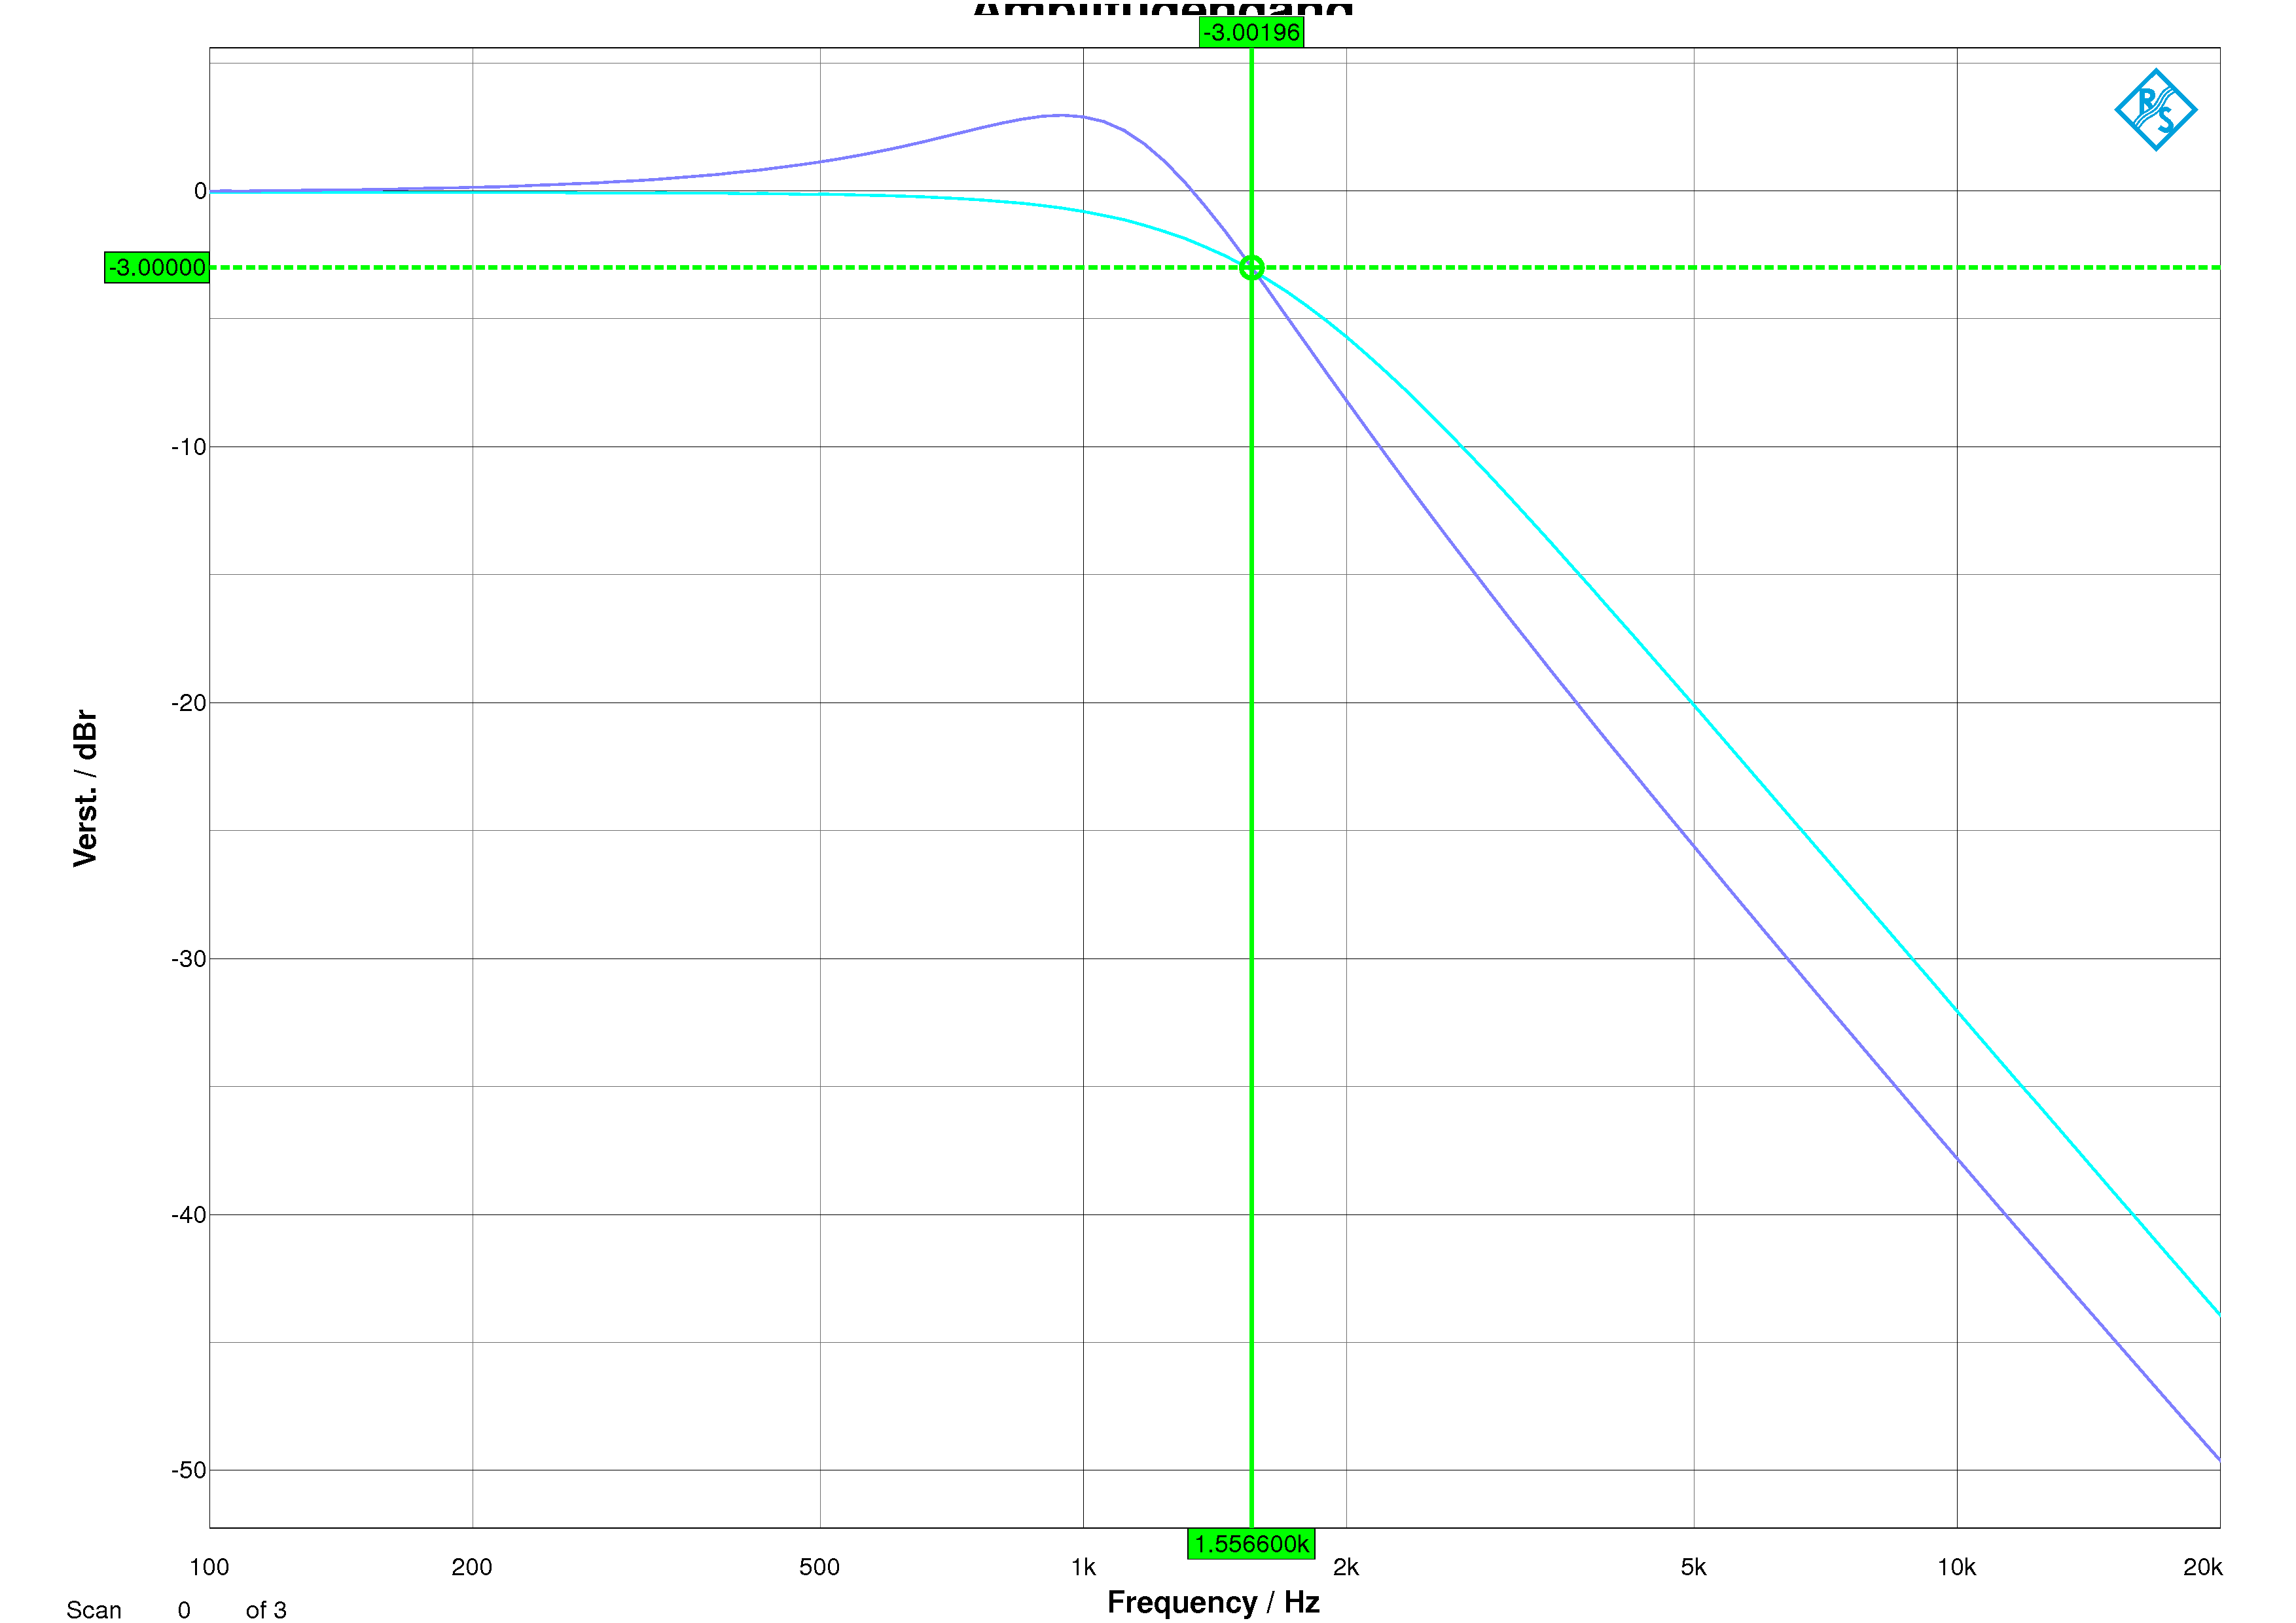
\includegraphics[width=0.60\linewidth]{Bilder/ImLabor/Amplitudengang_2_2_Tscheby_TP}
\caption{Amplitudengang Butterworth- und Tschebyscheff-Tiefpass mit Marker bei Tschebyscheff}
\label{fig:Amplitudengang_2_2_Tscheby_TP}
\end{figure}

\begin{figure}[h]
\centering
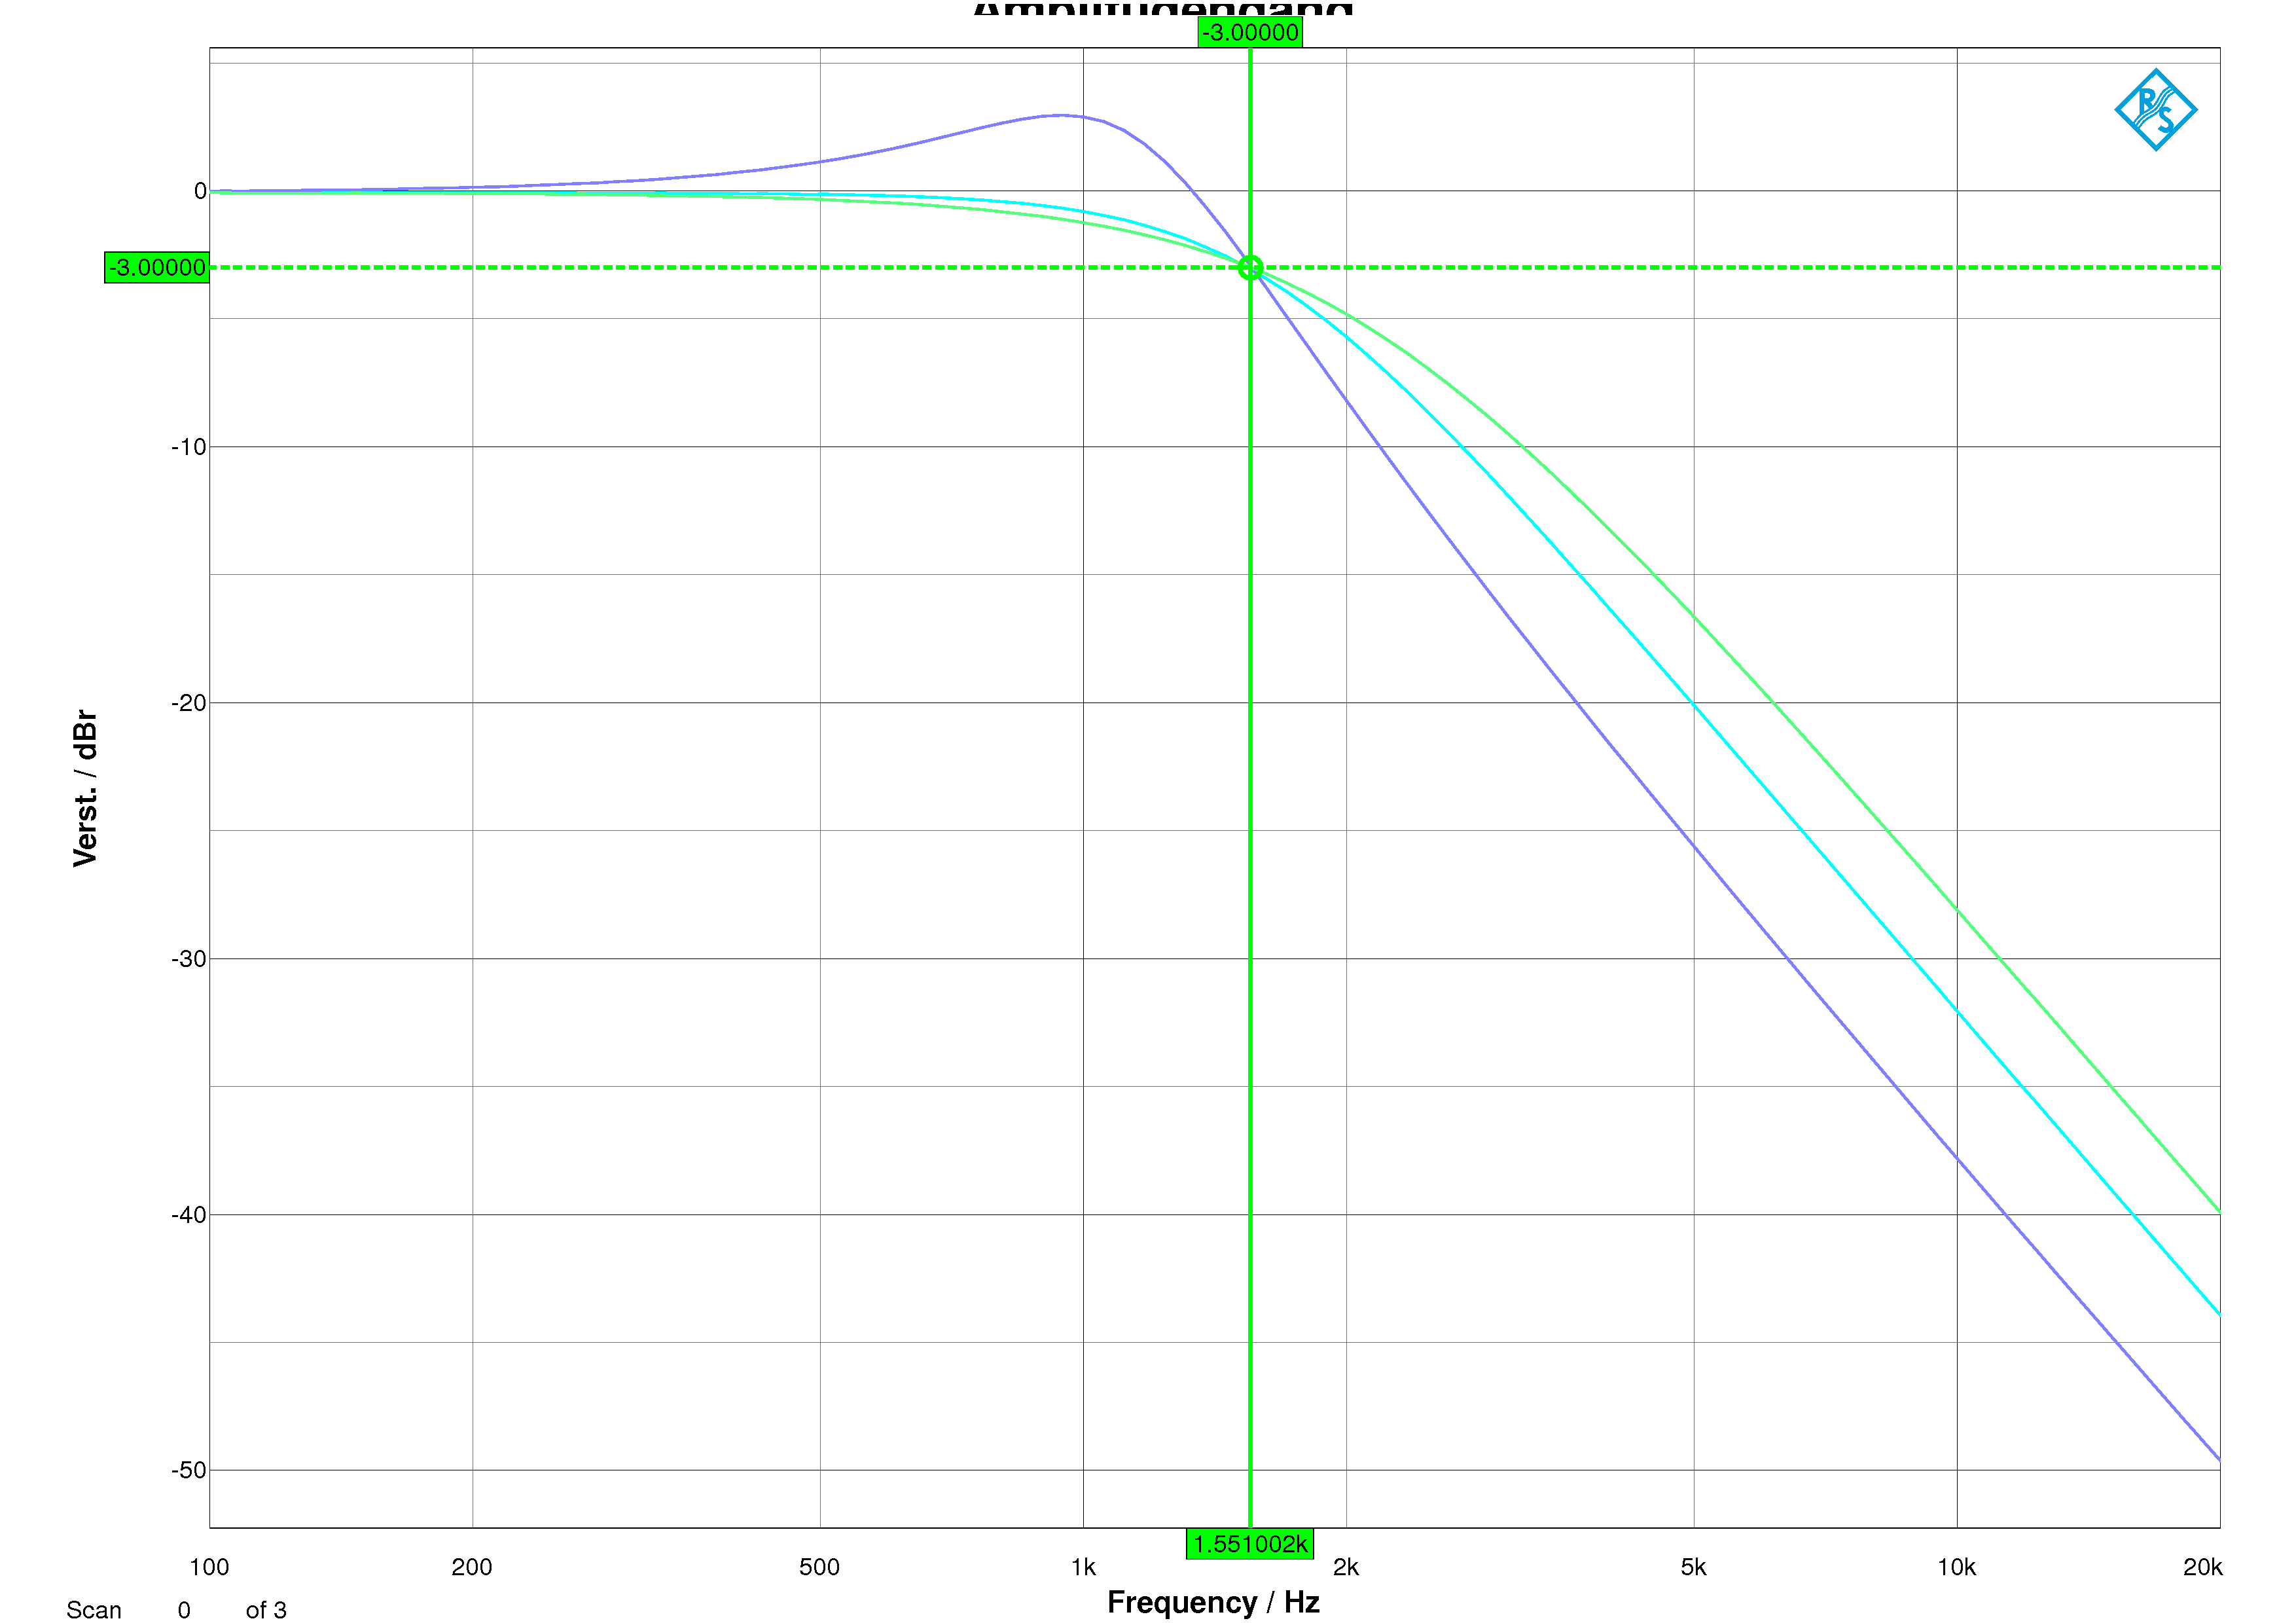
\includegraphics[width=0.60\linewidth]{Bilder/ImLabor/Amplitudengang_2_3_Bessel_TP_Alle}
\caption{Amplitudengang Butterworth-, Tschebyscheff- und Bessel-Tiefpass mit Marker bei Bessel}
\label{fig:Amplitudengang_2_3_Bessel_TP_Alle}
\end{figure}

\newpage
\newpage

\subsubsection{Hochpässe}

\begin{figure}[h]
\centering
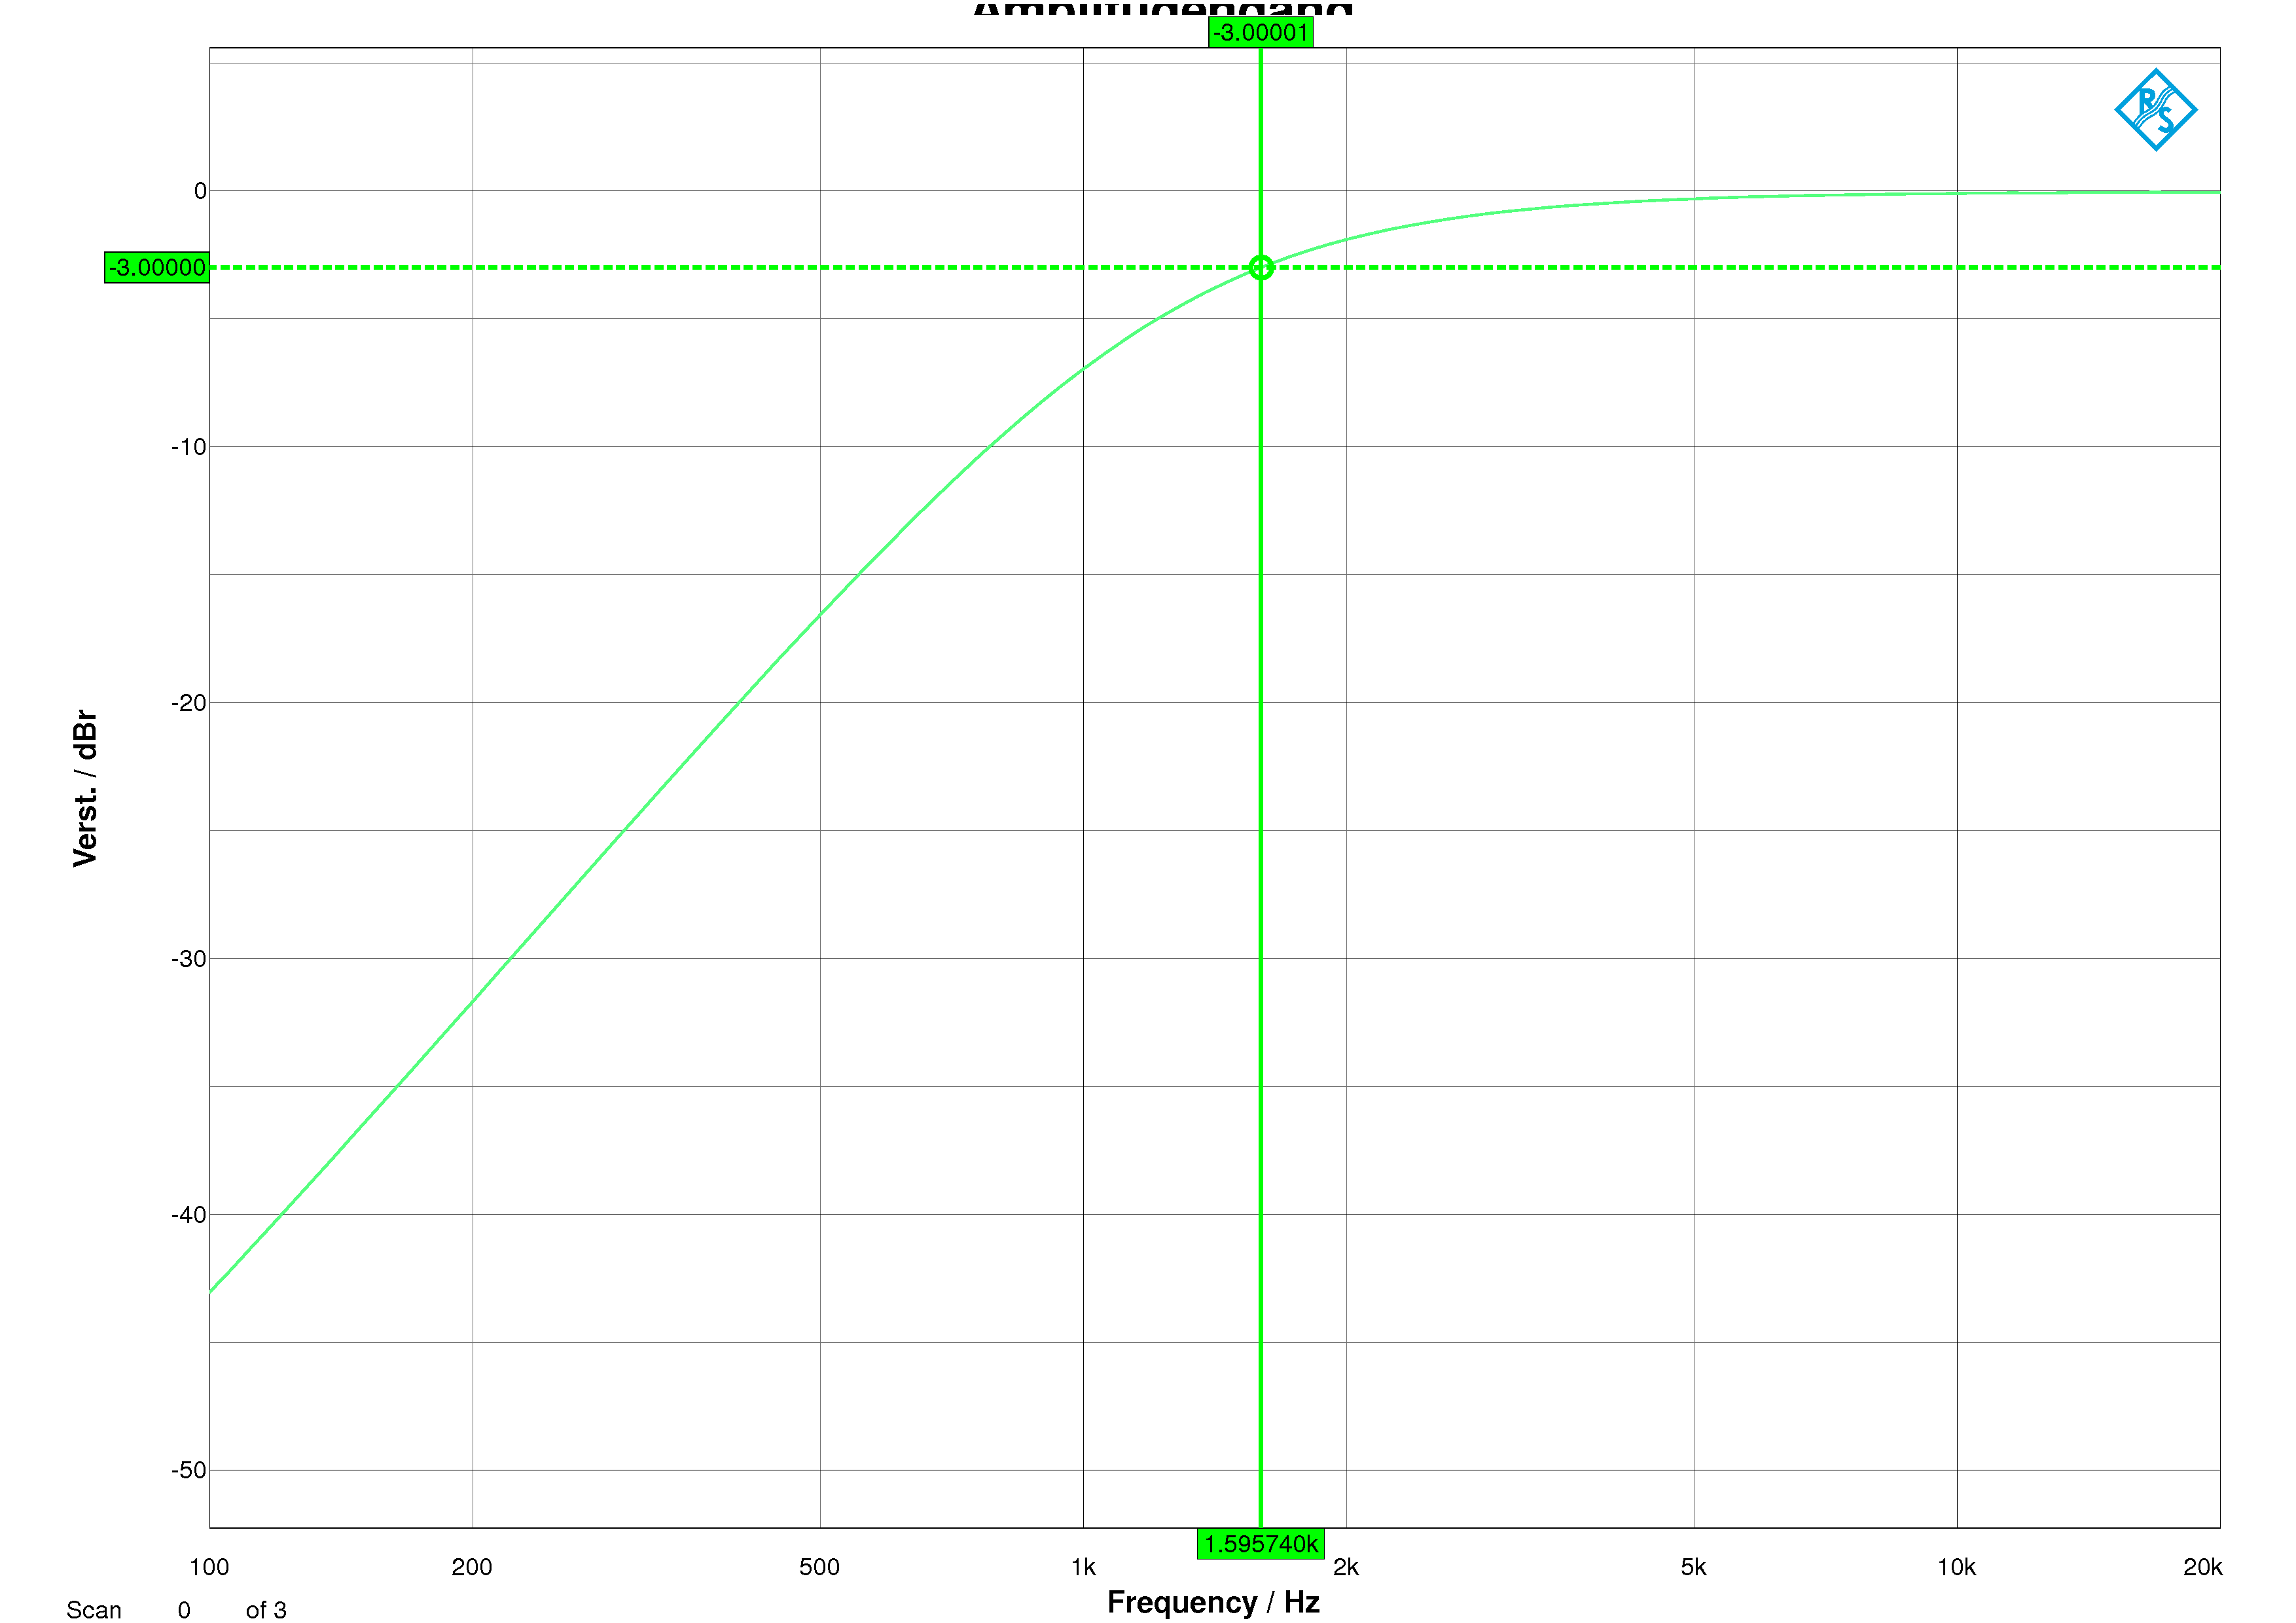
\includegraphics[width=0.60\linewidth]{Bilder/ImLabor/Amplitudengang_1_1_Butter_HP}
\caption{Amplitudengang Butterworth-Hochpass mit Marker}
\label{fig:Amplitudengang_1_1_Butter_HP}
\end{figure}

\begin{figure}[h]
\centering
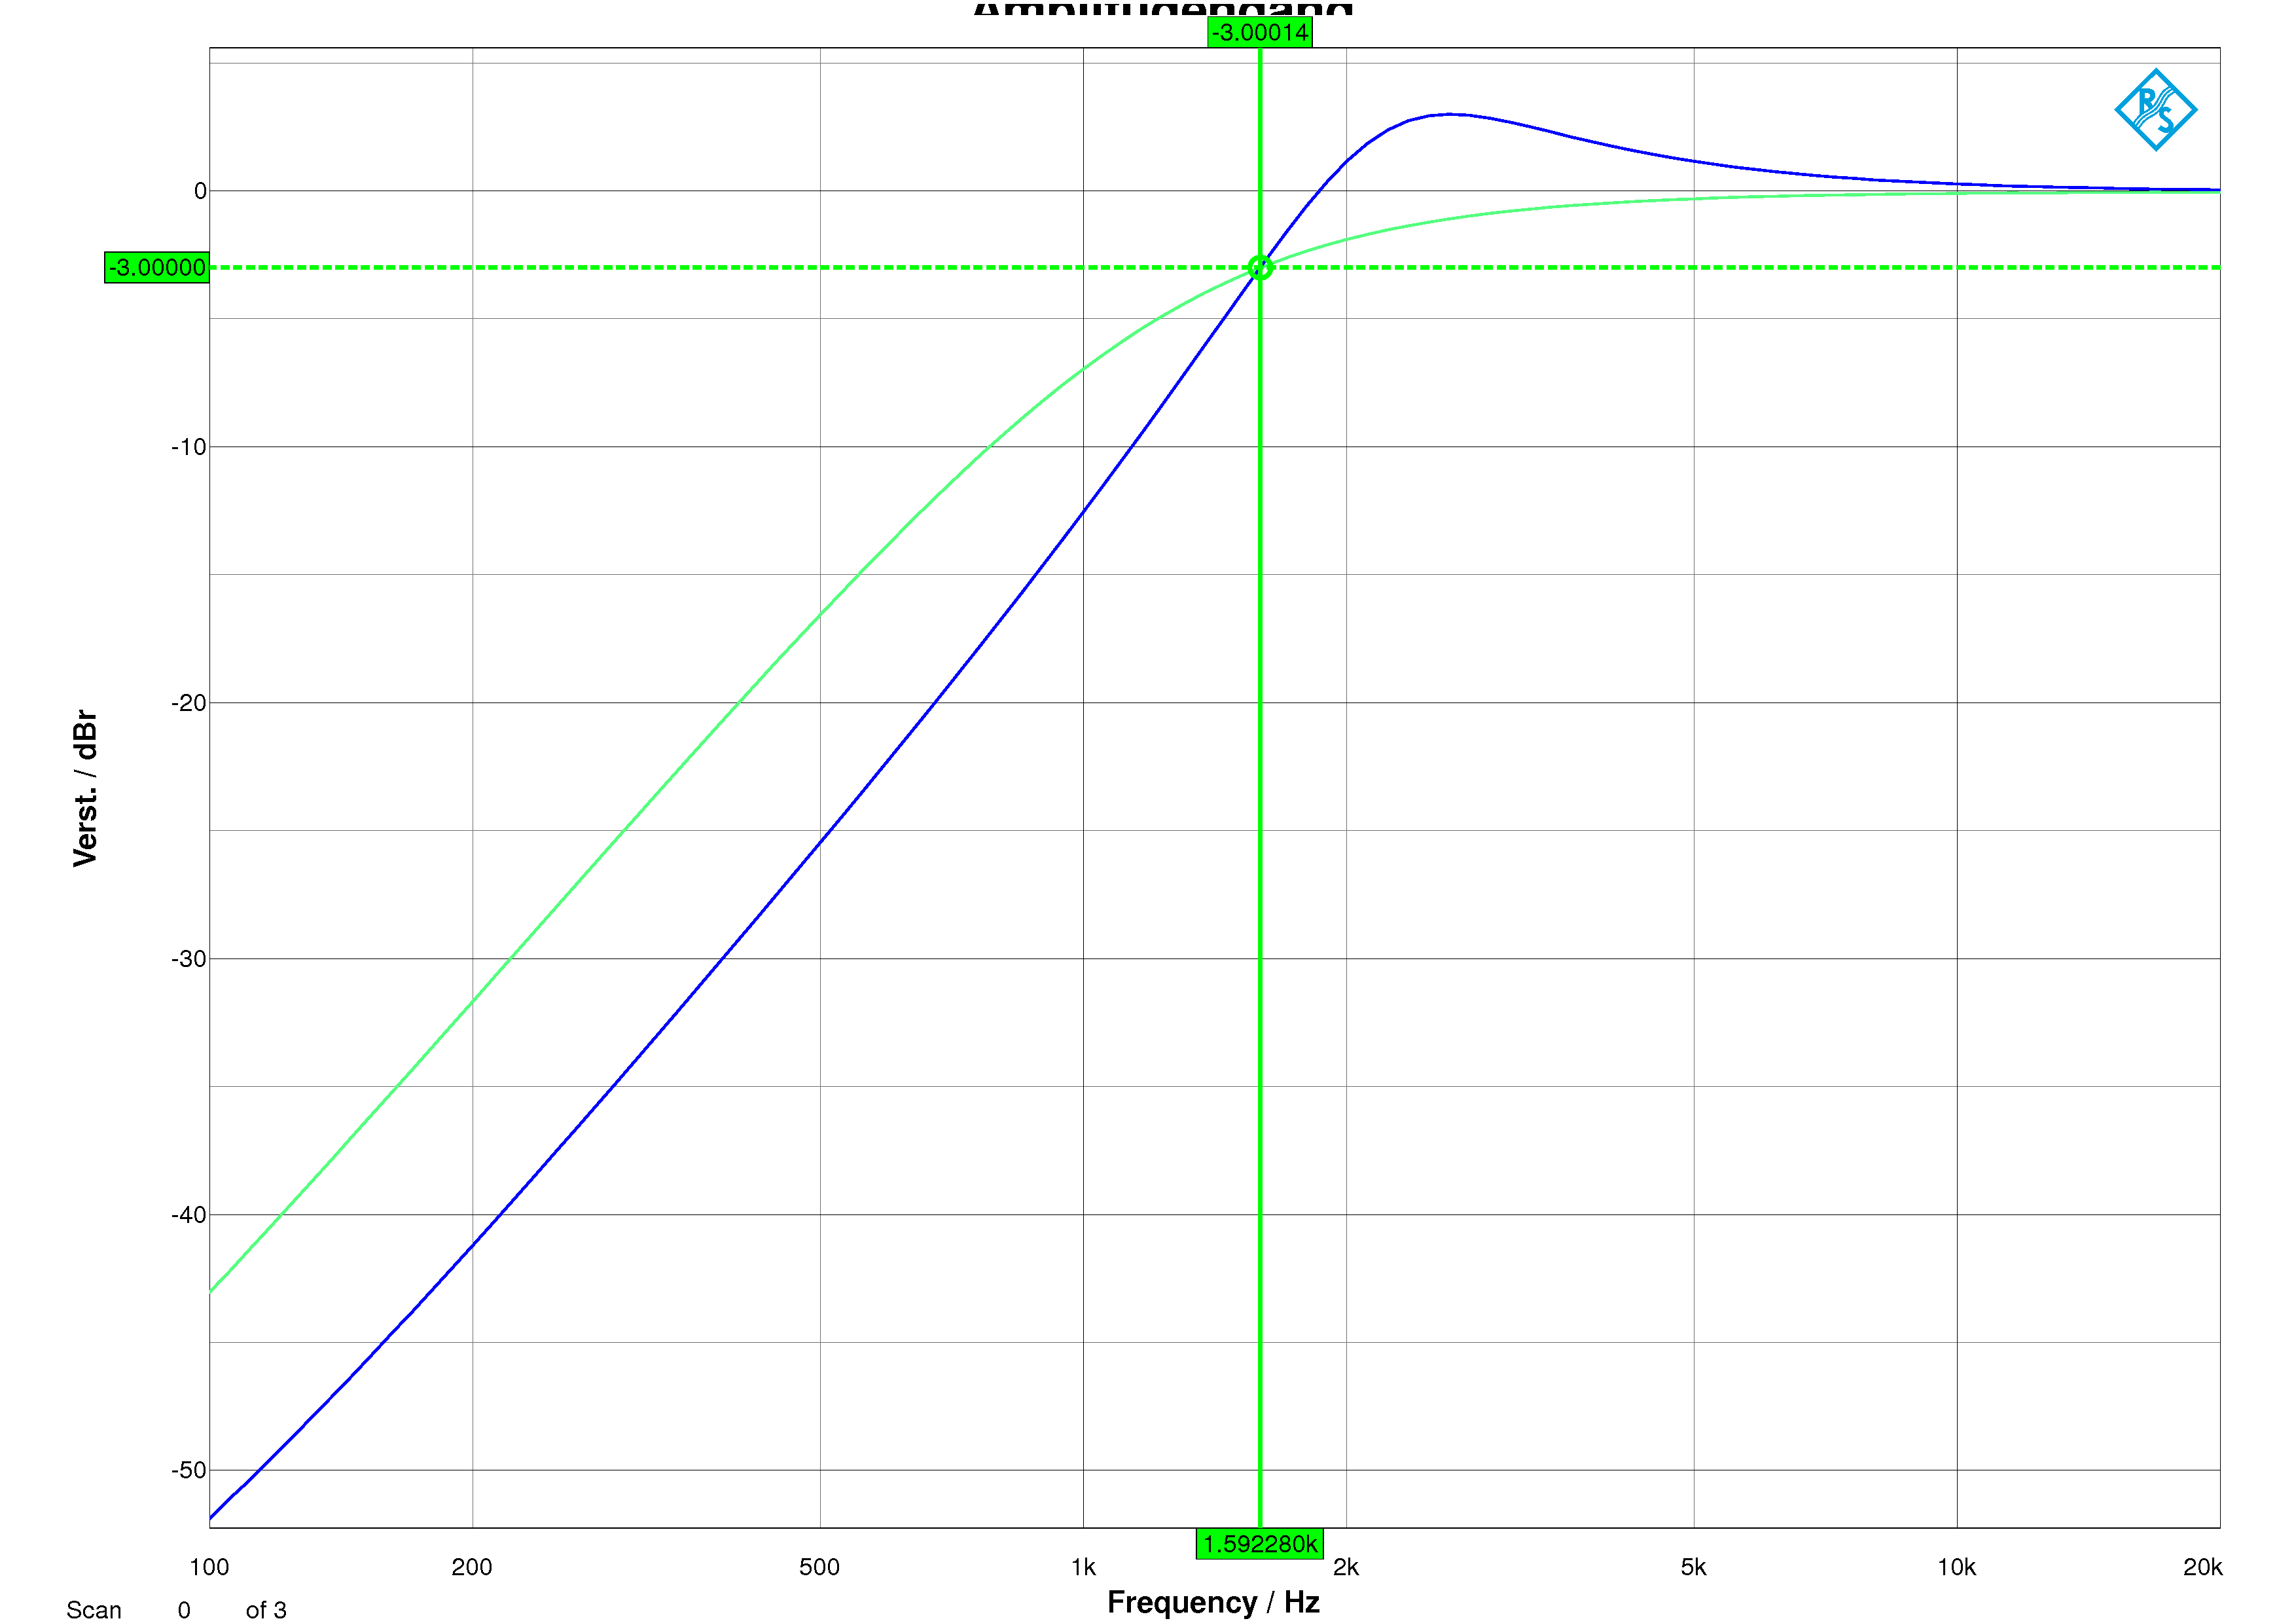
\includegraphics[width=0.60\linewidth]{Bilder/ImLabor/Amplitudengang_1_2_Tscheby_HP}
\caption{Amplitudengang Butterworth- und Tschebyscheff-Hochpass mit Marker bei Tschebyscheff}
\label{fig:Amplitudengang_1_2_Tscheby_HP}
\end{figure}

\begin{figure}[h]
\centering
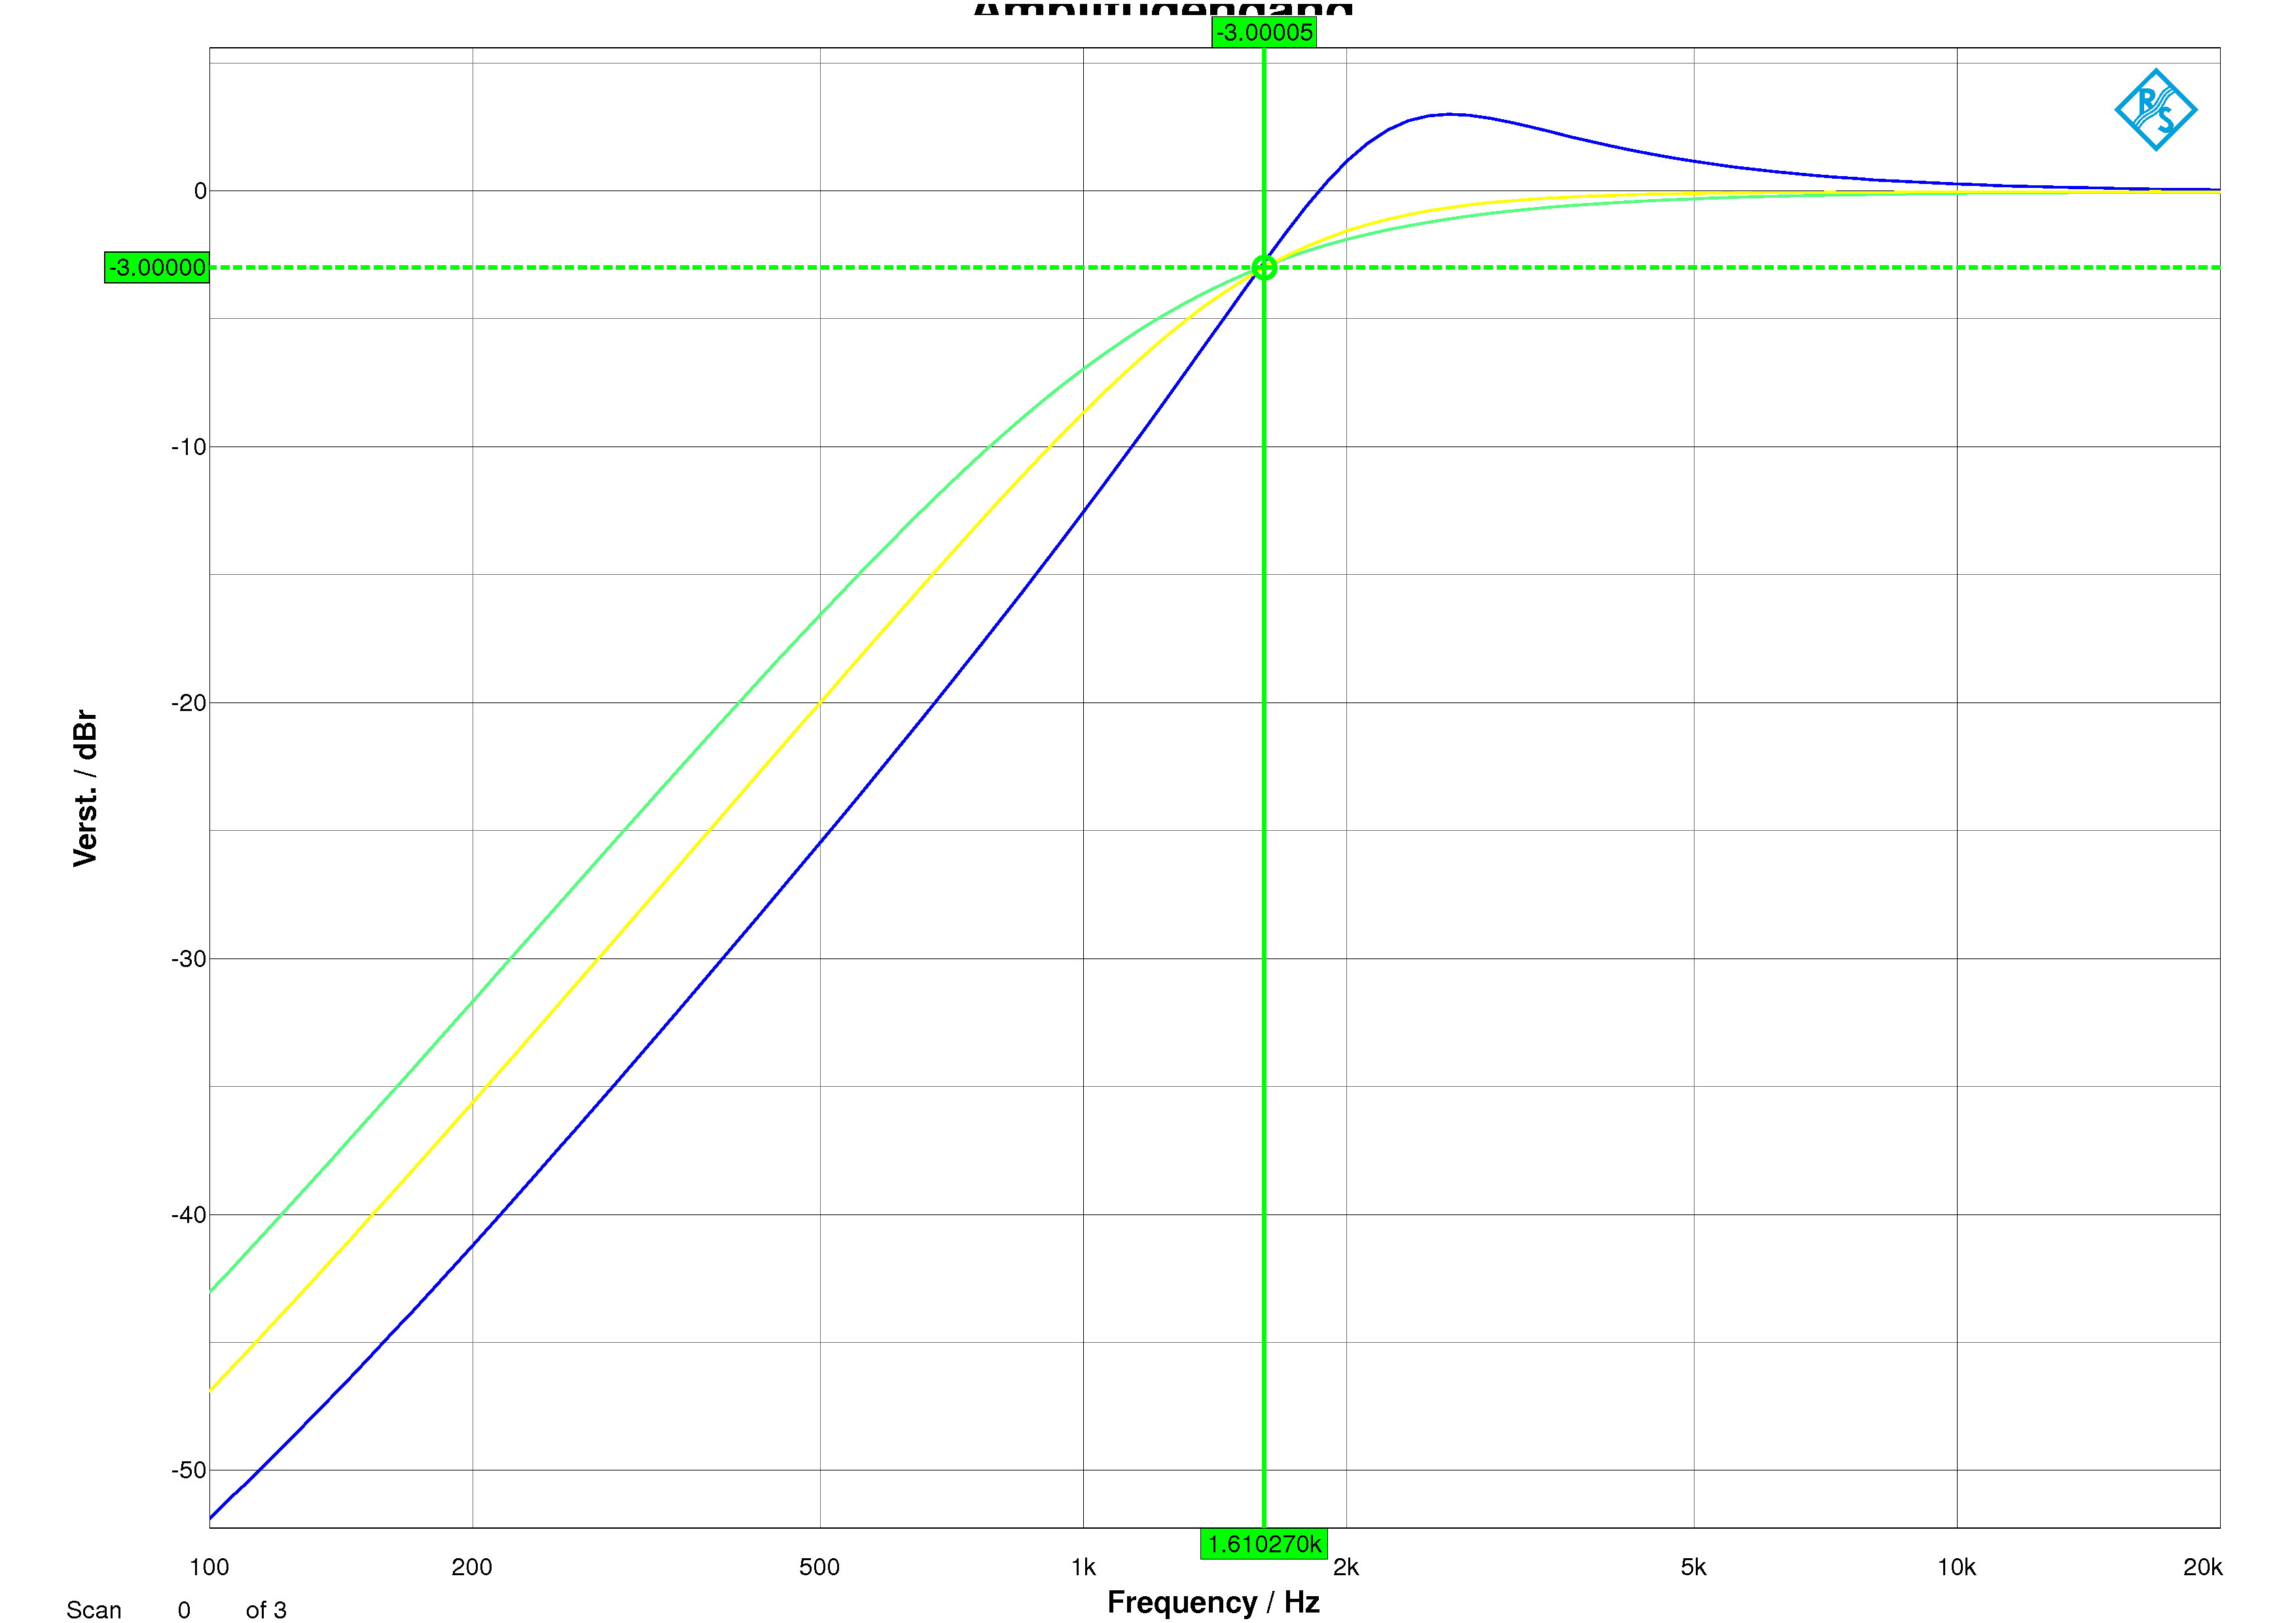
\includegraphics[width=0.60\linewidth]{Bilder/ImLabor/Amplitudengang_1_3_Bessel_HP_Alle}
\caption{Amplitudengang Butterworth-, Tschebyscheff- und Bessel-Hochpass mit Marker bei Bessel}
\label{fig:Amplitudengang_1_3_Bessel_HP_Alle}
\end{figure}

\newpage

\subsubsection{Bandpass/Bandsperre}
\begin{figure}[h]
\centering
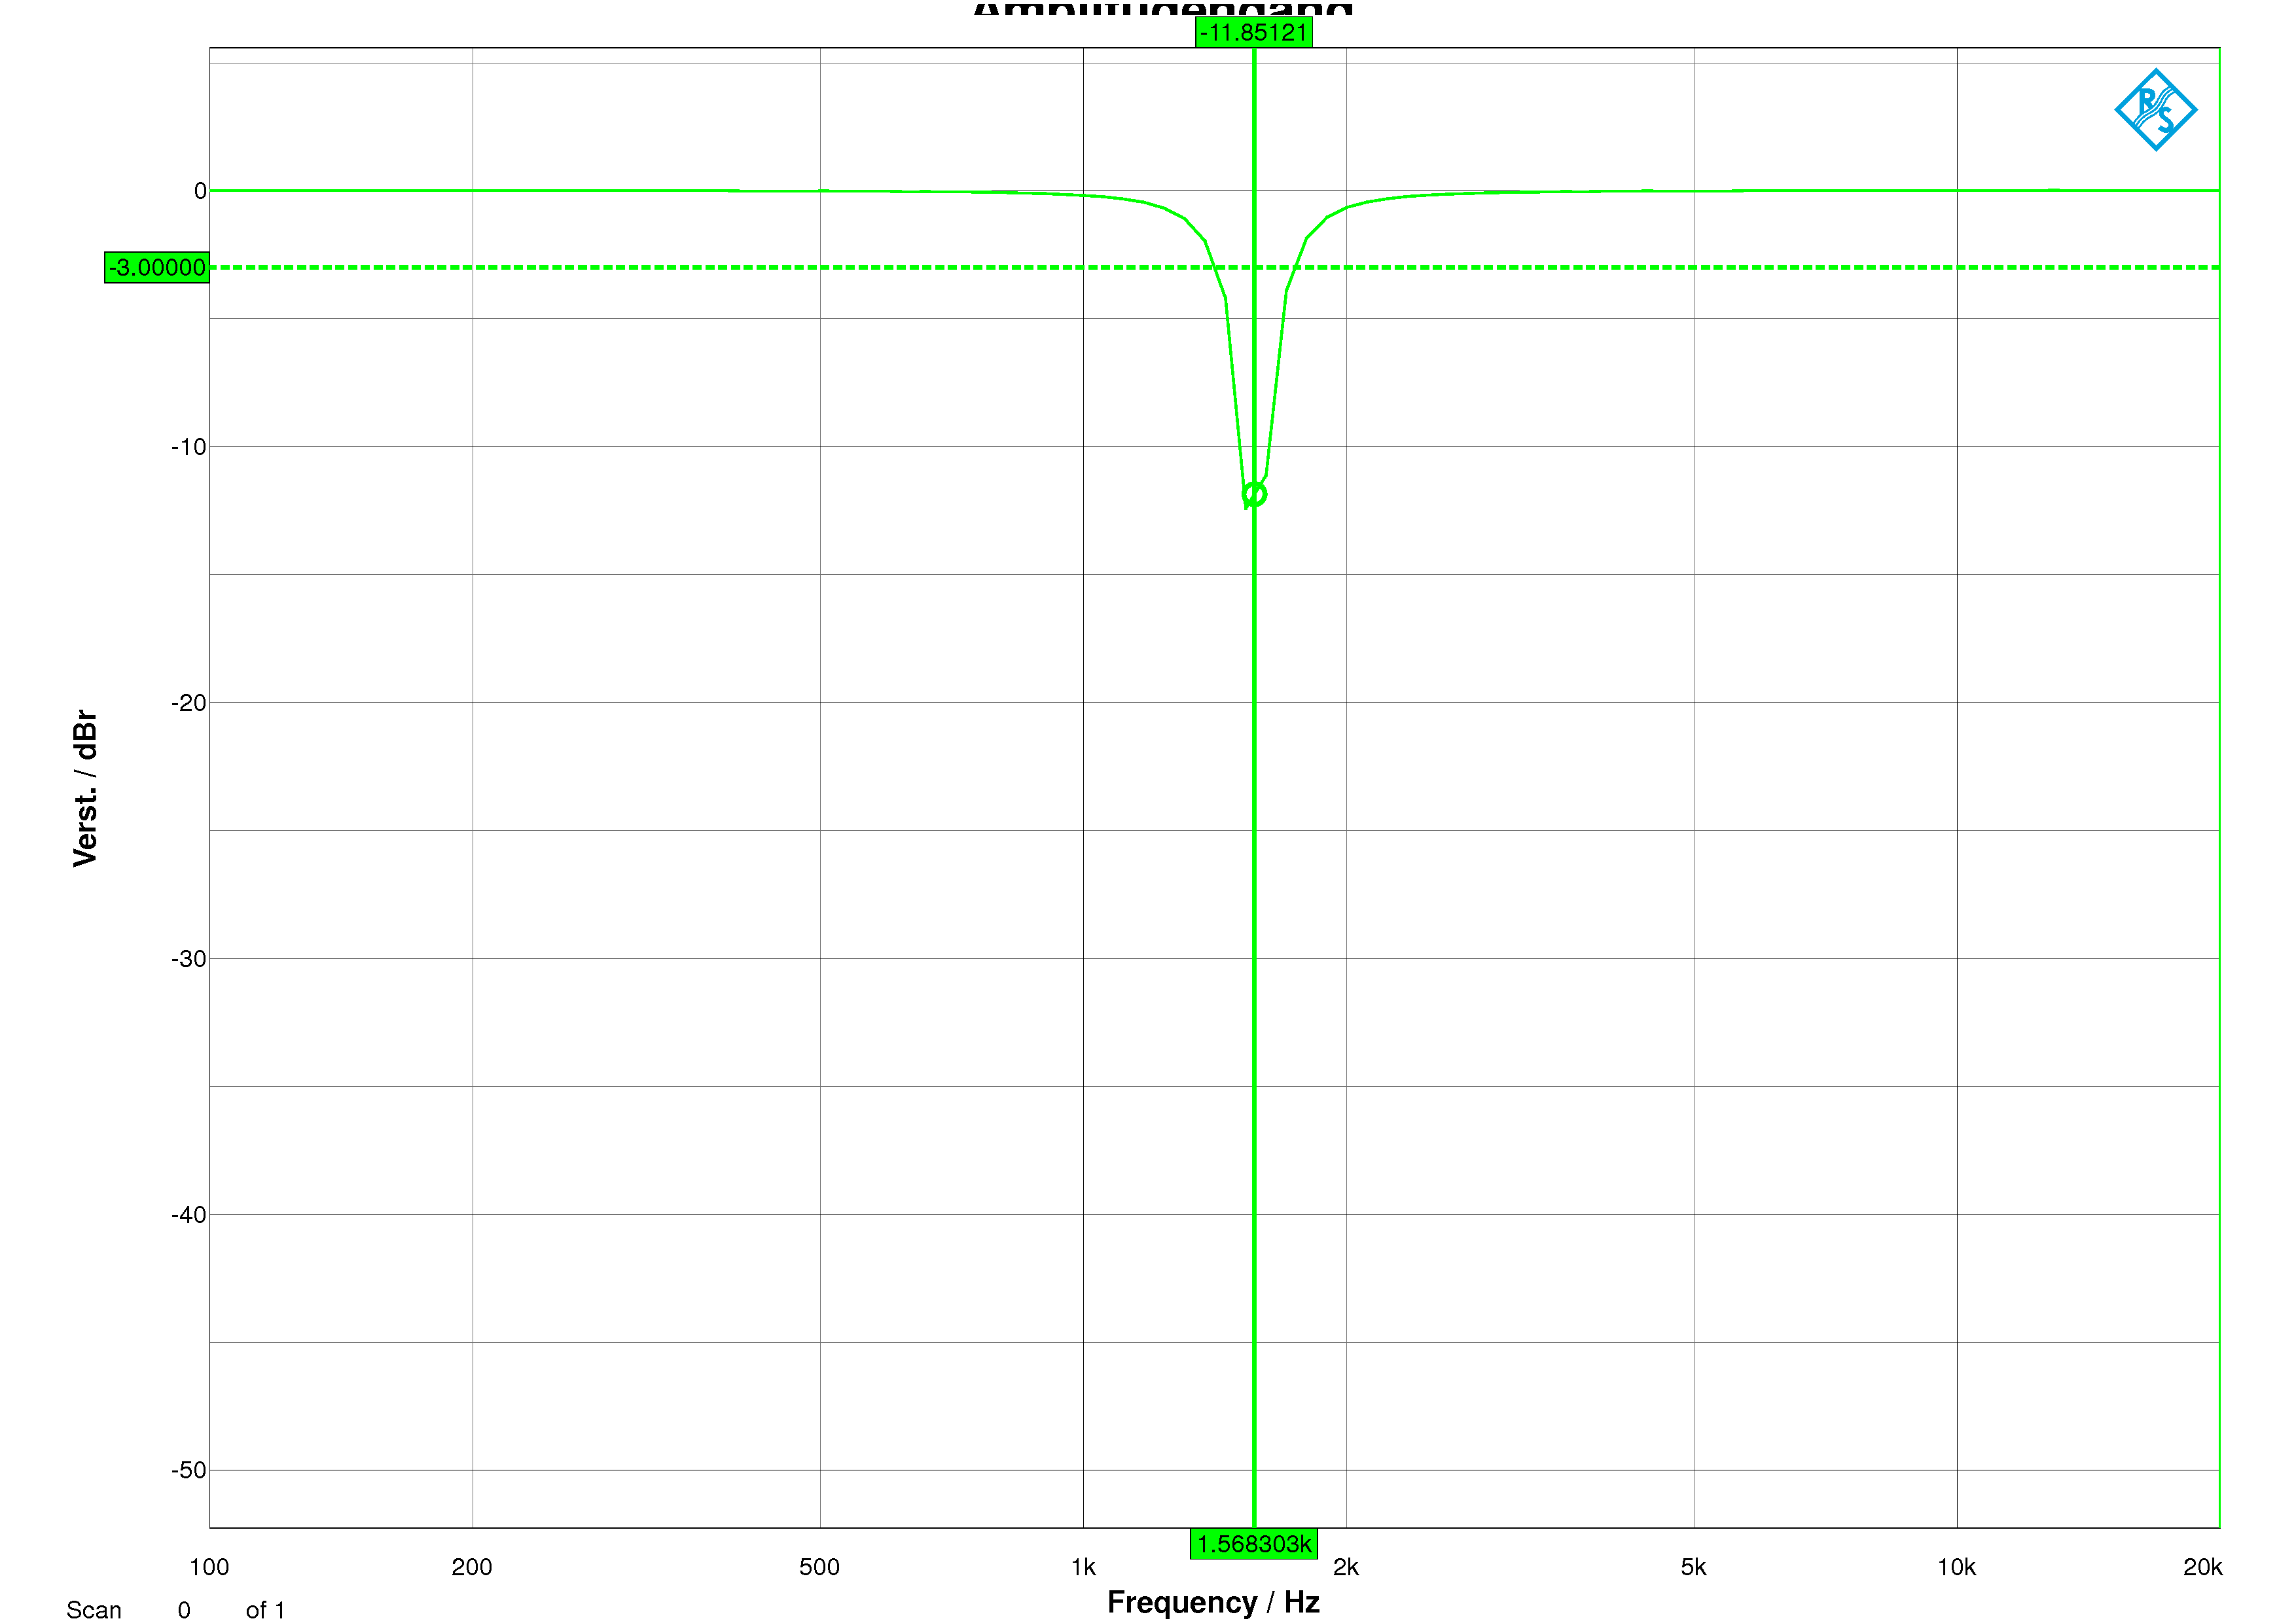
\includegraphics[width=0.60\linewidth]{Bilder/ImLabor/Amplitudengang_3_2_BS}
\caption{Amplitudengang Bandsperre mit Marker}
\label{fig:Amplitudengang_3_2_BS}
\end{figure}

\begin{figure}[h]
\centering
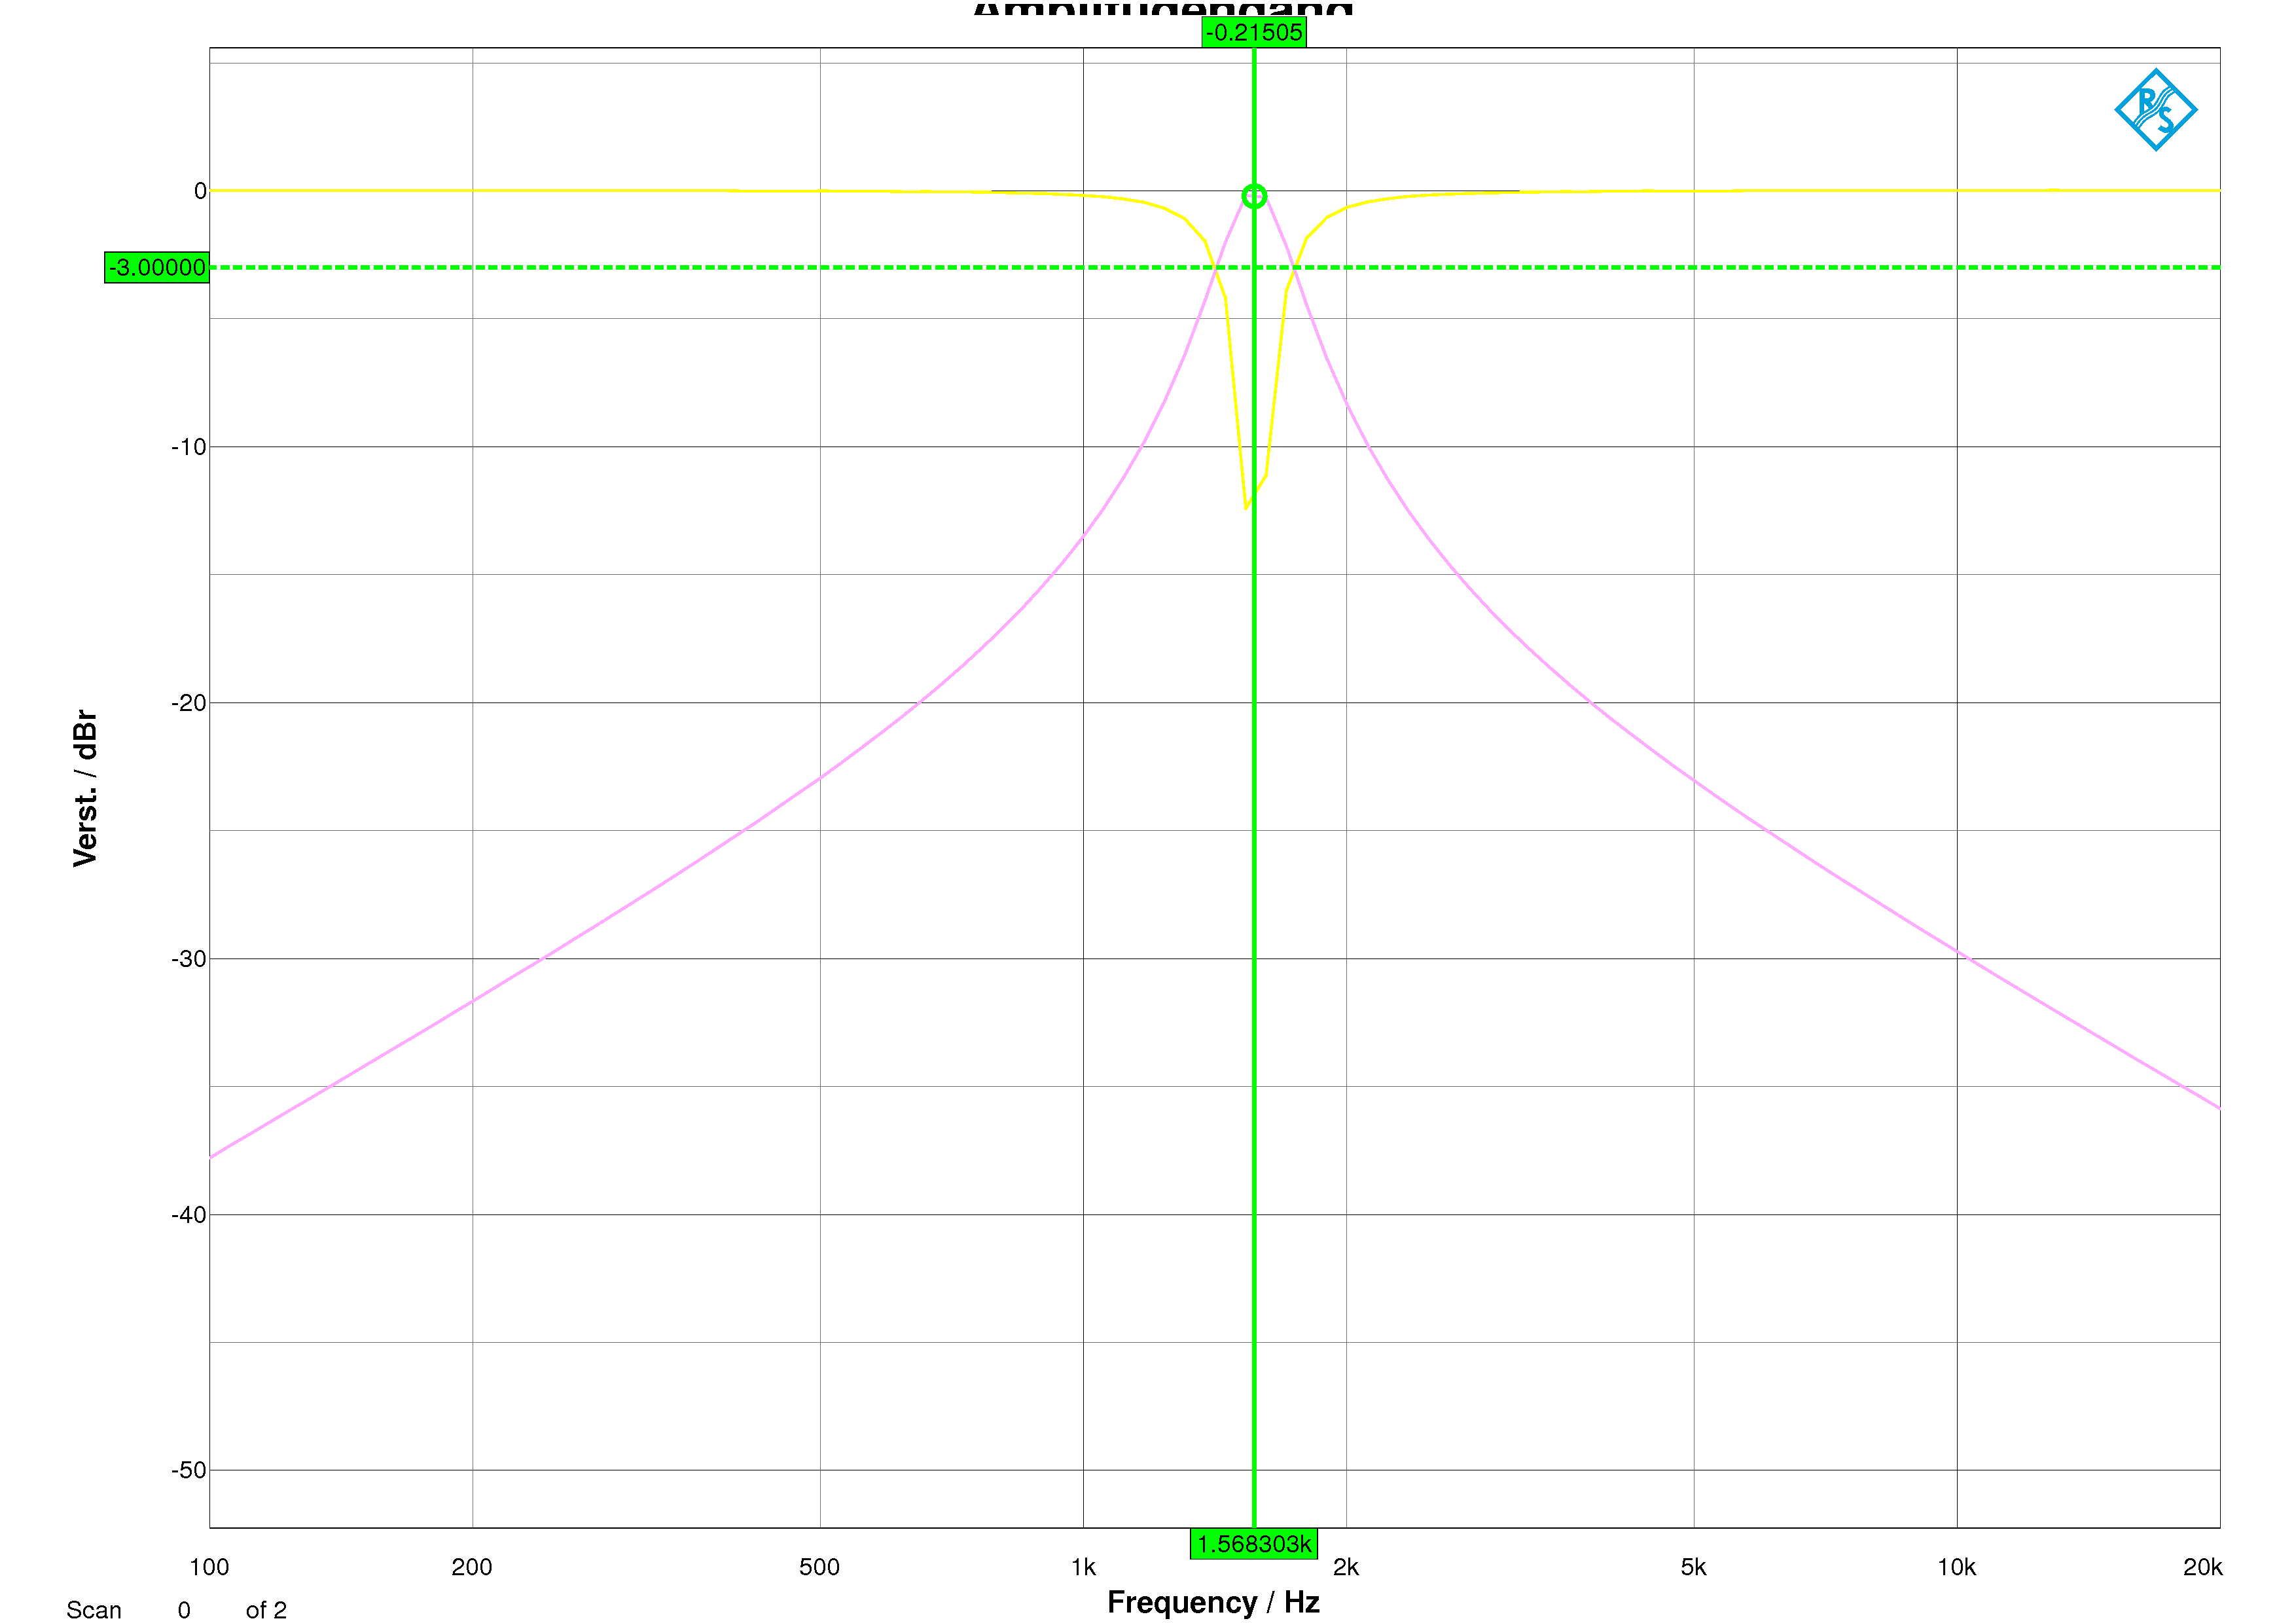
\includegraphics[width=0.60\linewidth]{Bilder/ImLabor/Amplitudengang_3_3_BP_BS}
\caption{Amplitudengang Bandsperre und Bandpass mit Maker beim Bandpass}
\label{fig:Amplitudengang_3_3_BP_BS}
\end{figure}

\newpage

\subsection{Phasengänge Tiefpässe}

\begin{figure}[h]
\centering
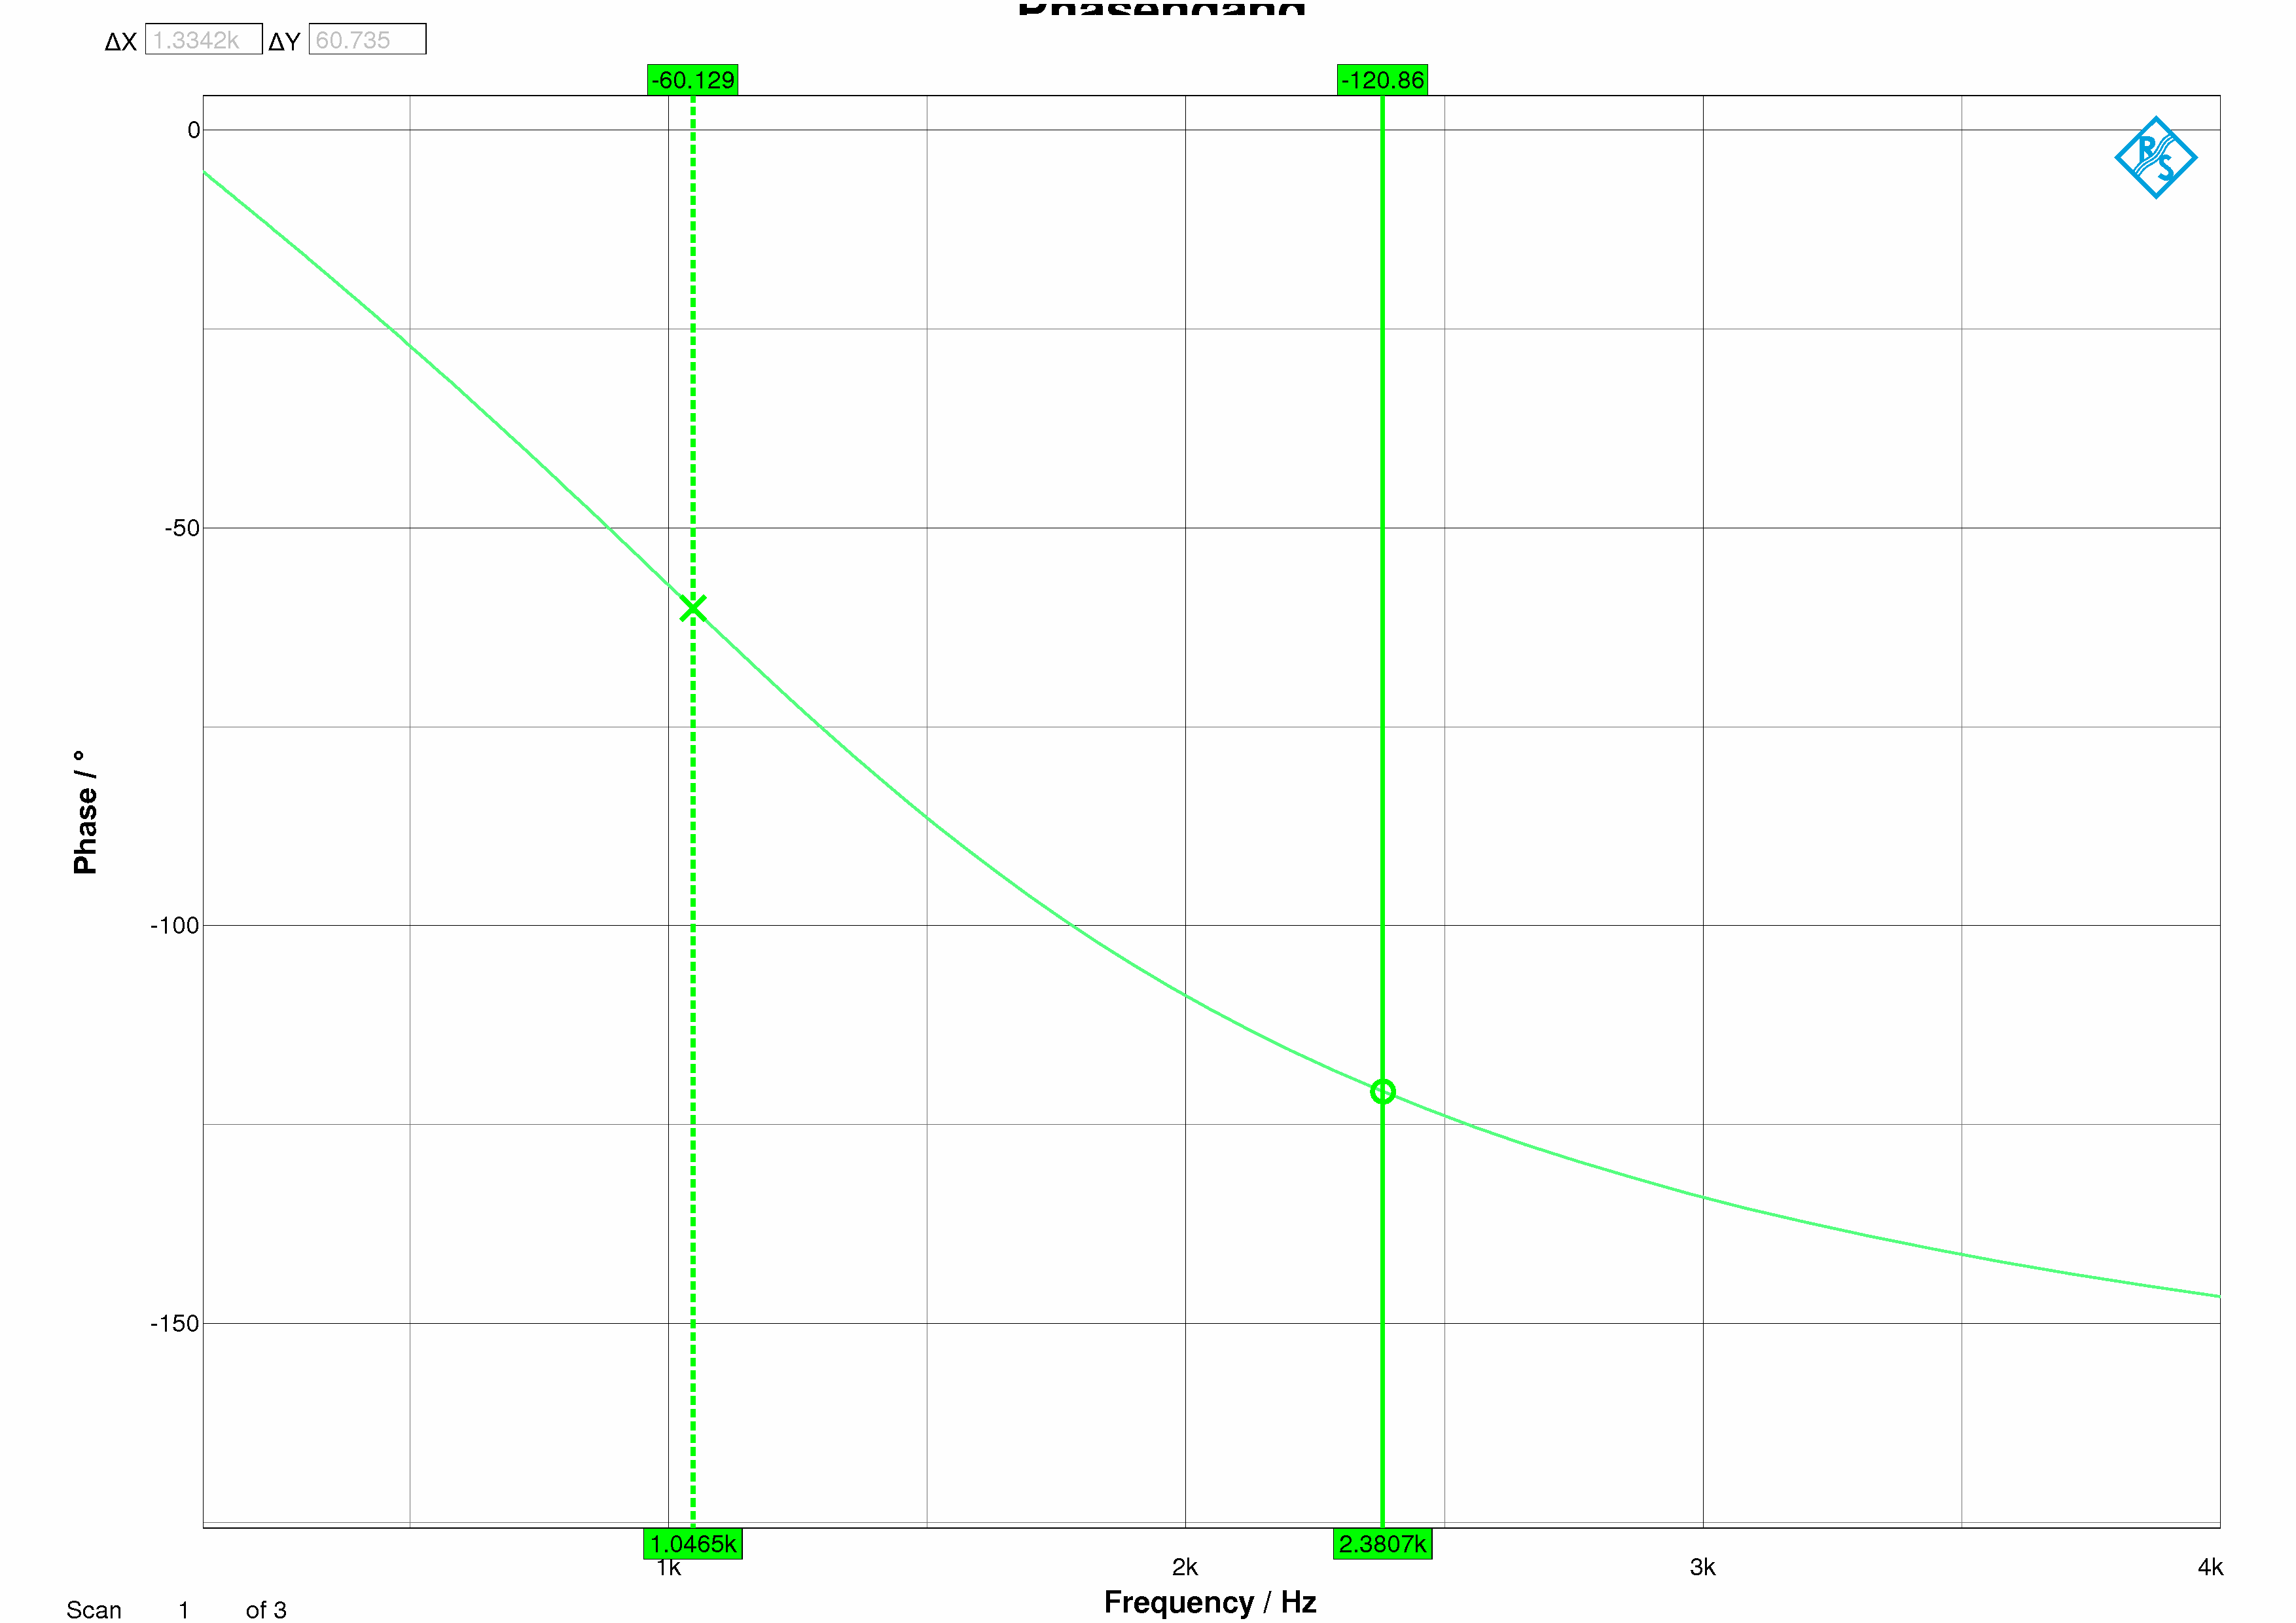
\includegraphics[width=0.60\linewidth]{Bilder/ImLabor/Phasengang_4_1_Butter_TP}
\caption{Phasengang Butterworth-Tiefpass mit Markern}
\label{fig:Phasengang_4_1_Butter_TP}
\end{figure}

\begin{figure}[h]
\centering
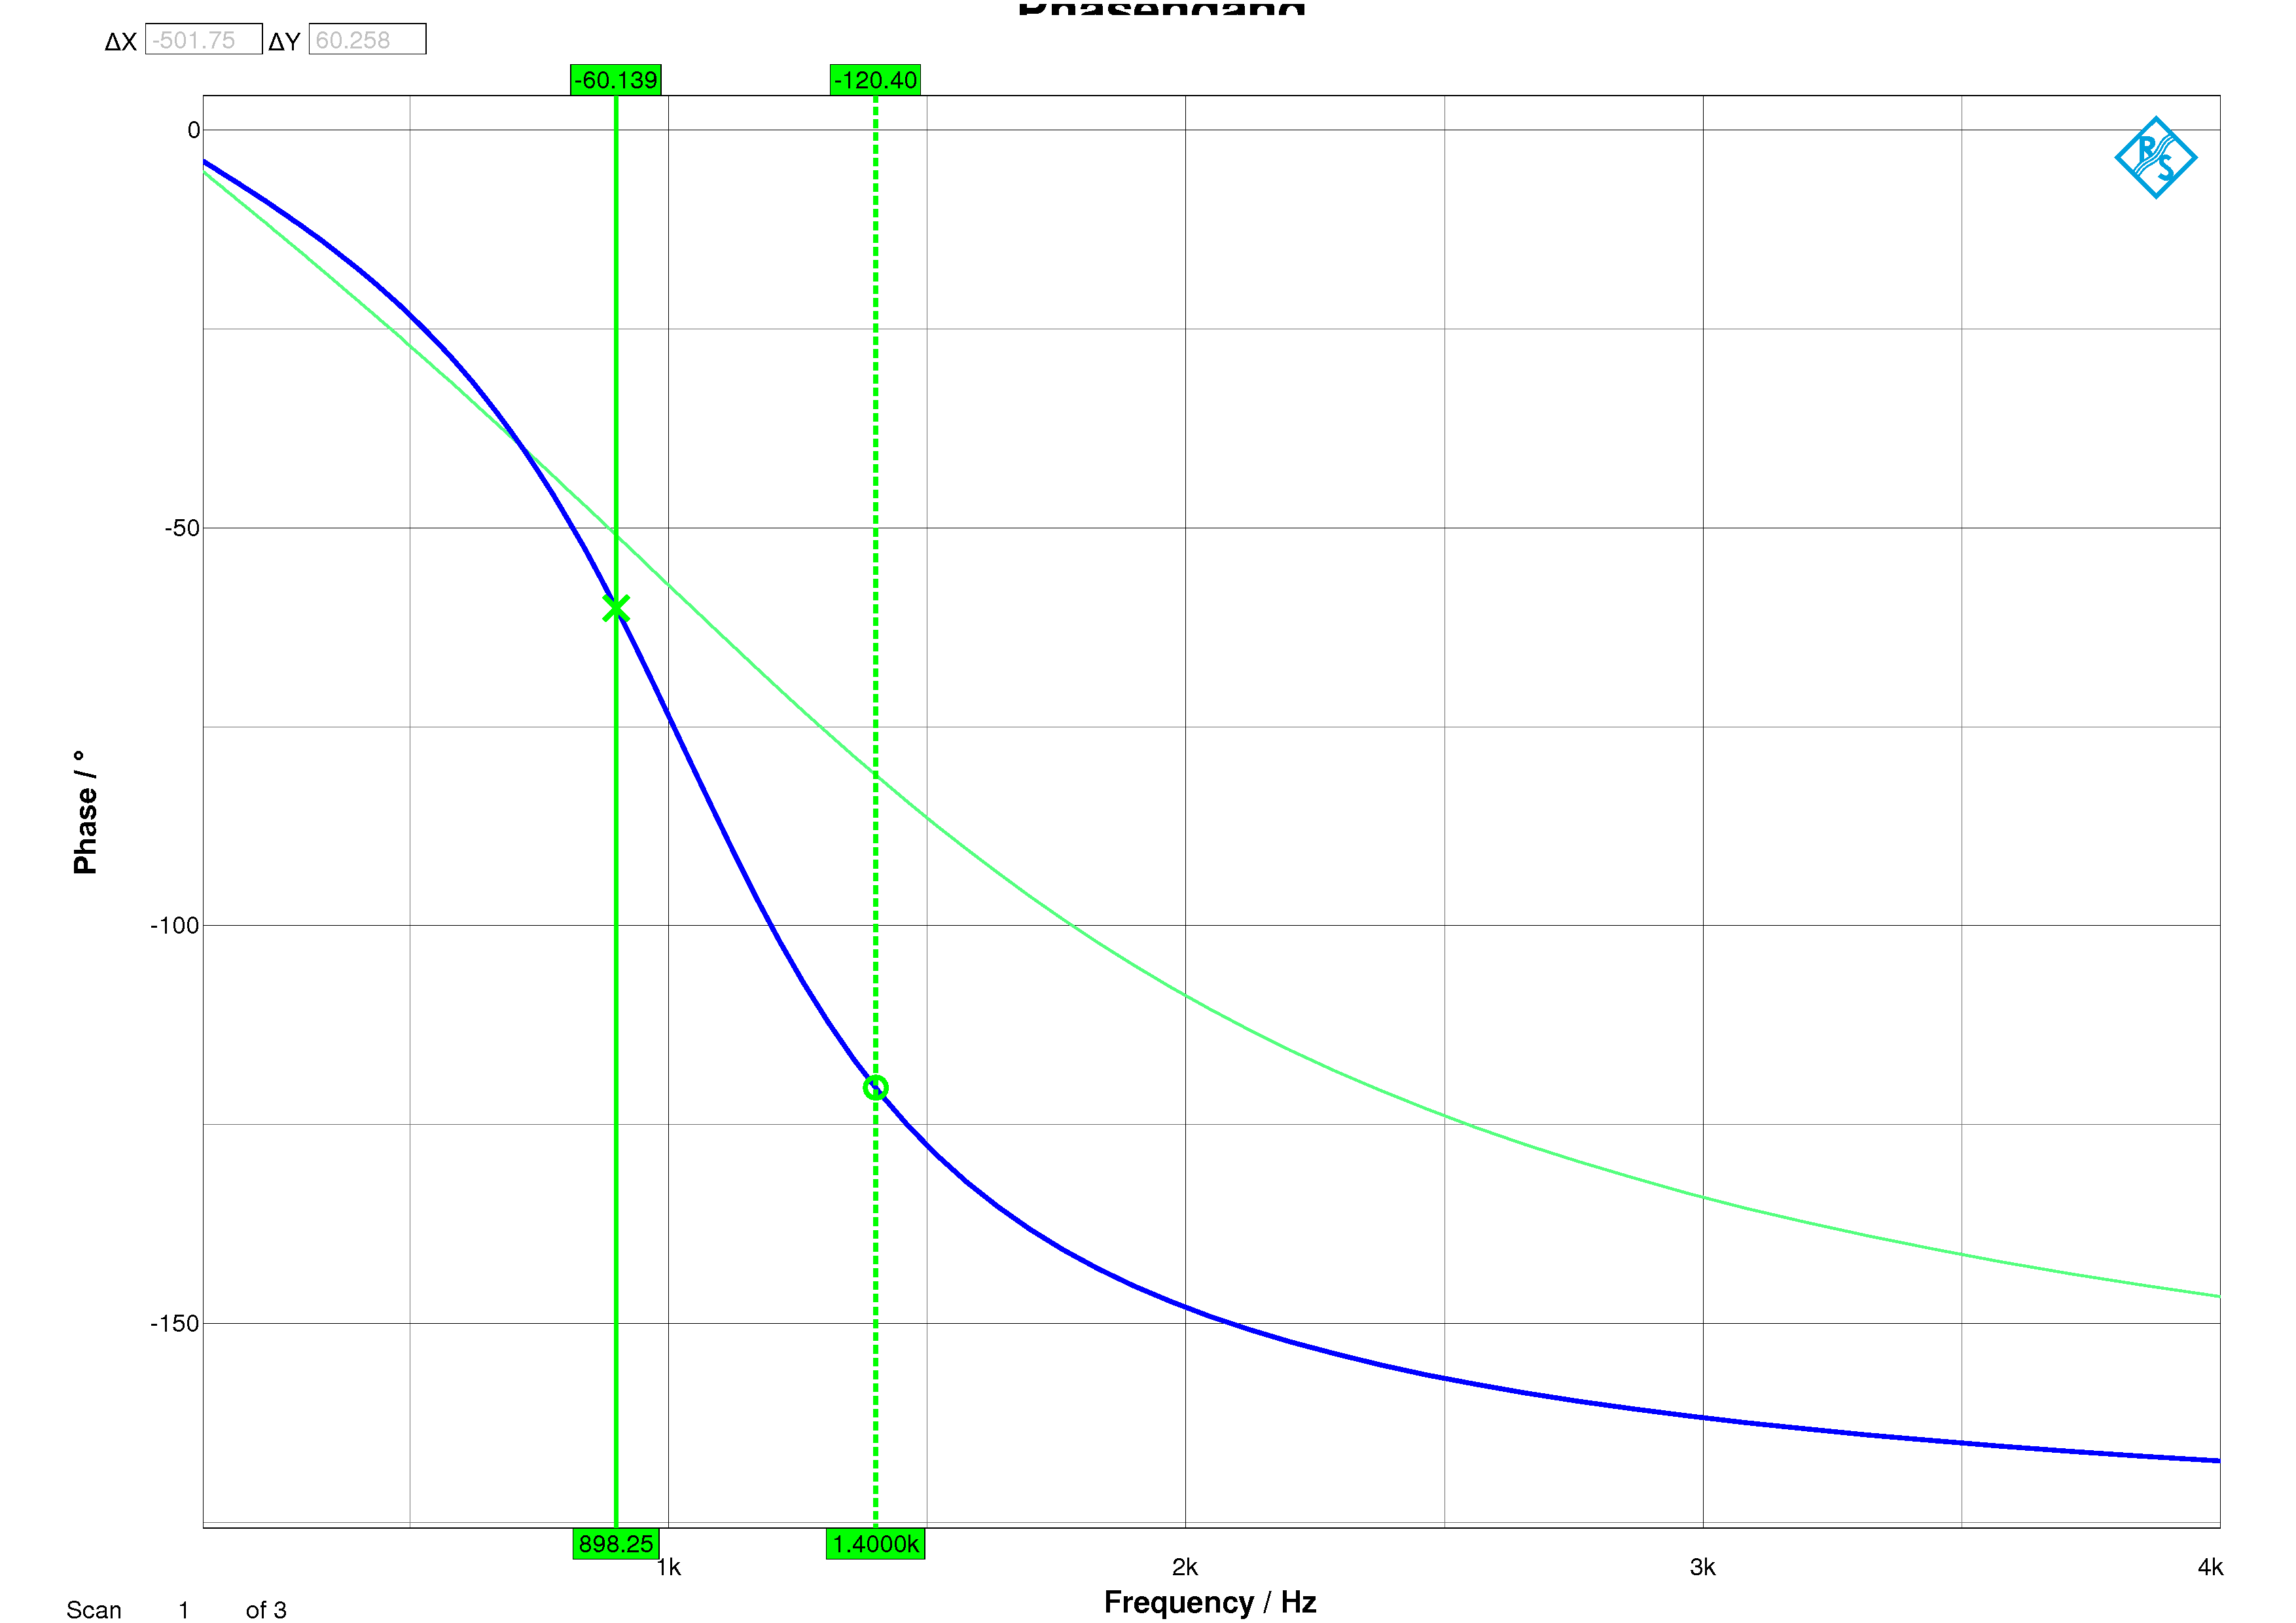
\includegraphics[width=0.60\linewidth]{Bilder/ImLabor/Phasengang_4_2_Tscheby_TP}
\caption{Phasengang Butterworth- und Tschebyscheff-Tiefpass mit Markern bei Tschebyscheff}
\label{fig:Phasengang_4_2_Tscheby_TP}
\end{figure}

\begin{figure}[h]
\centering
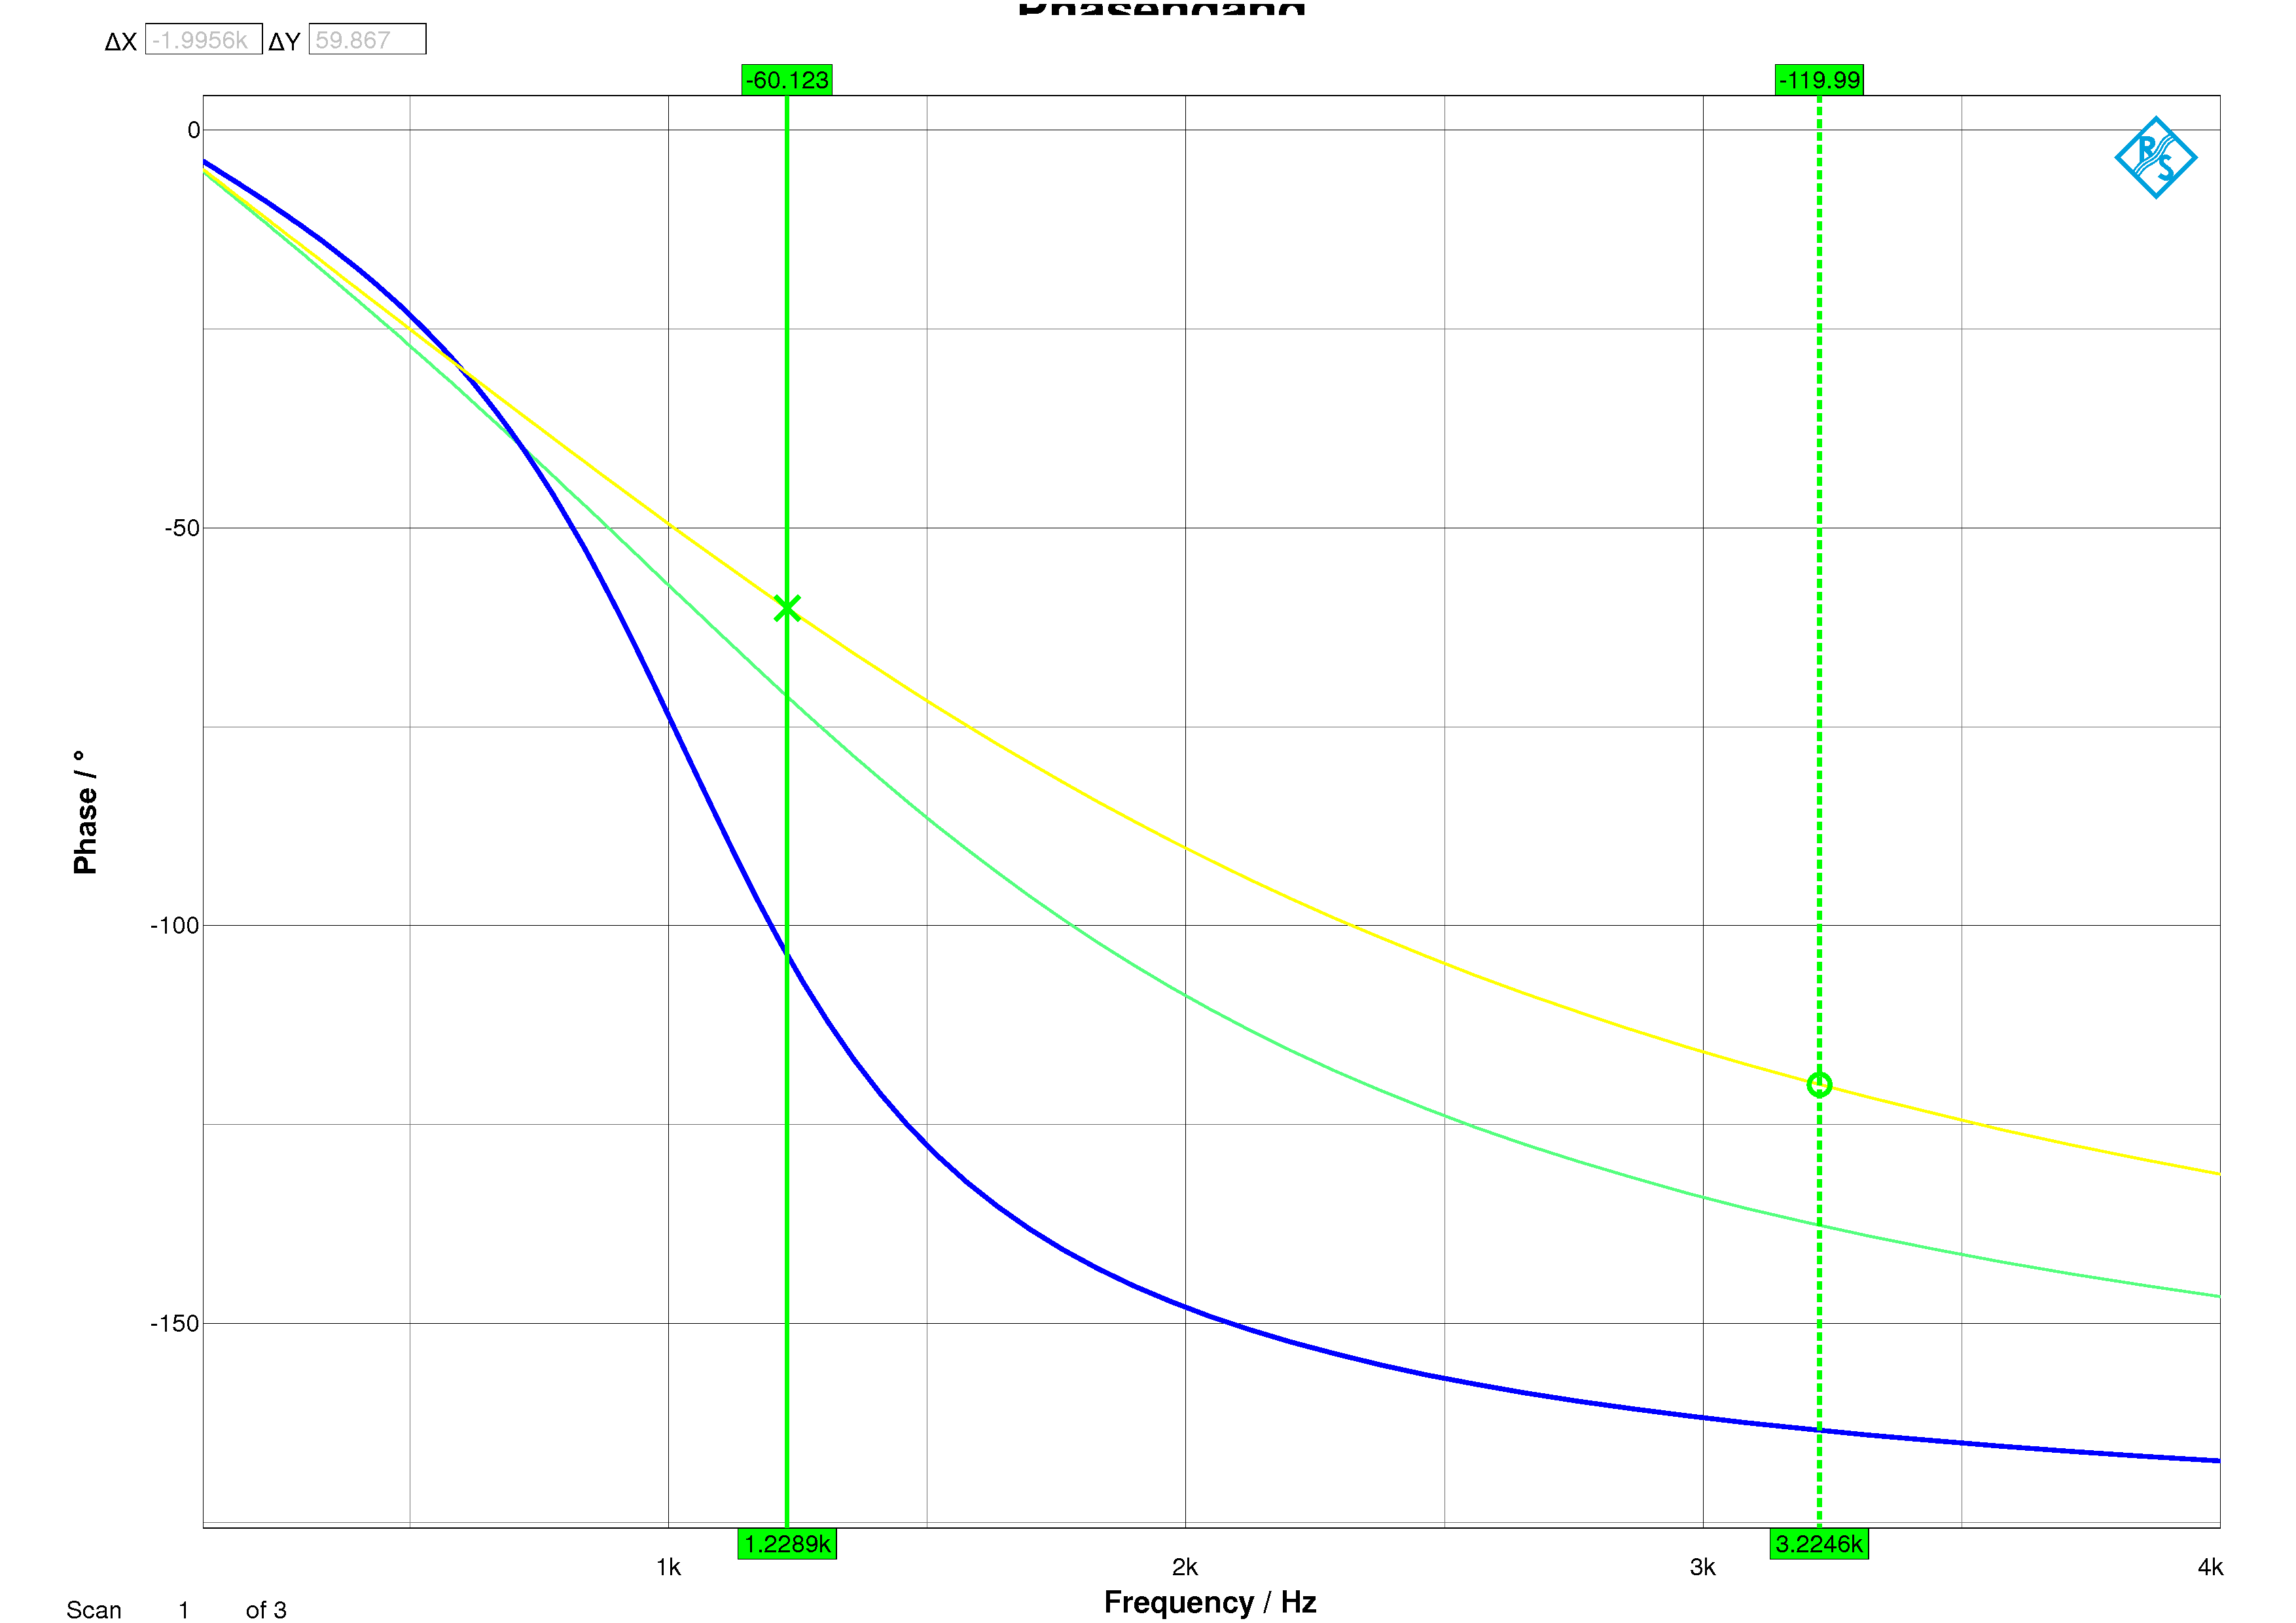
\includegraphics[width=0.60\linewidth]{Bilder/ImLabor/Phasengang_4_3_Bessel_TP_Alle}
\caption{Phasengang Butterworth-, Tschebyscheff- und Bessel-Tiefpass mit Markern bei Bessel}
\label{fig:Phasengang_4_3_Bessel_TP_Alle}
\end{figure}

\newpage

\subsection{Sprungantworten der Tiefpässe}
\subsubsection{Butterworth}

\begin{figure}[h]
	\centering
	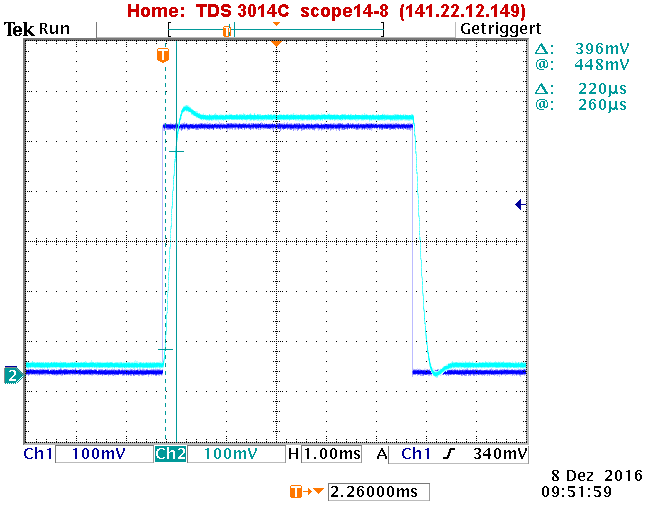
\includegraphics[width=0.60\linewidth]{Bilder/ImLabor/Sprungantwort_5_8_Butter_Anstiegszeit}
	\caption{Sprungantwort Butterworth: Messung der Anstiegszeit}
	\label{fig:Sprungantwort_5_8_Butter_Anstiegszeit_Anhang}
\end{figure}

\begin{figure}[h]
	\centering
	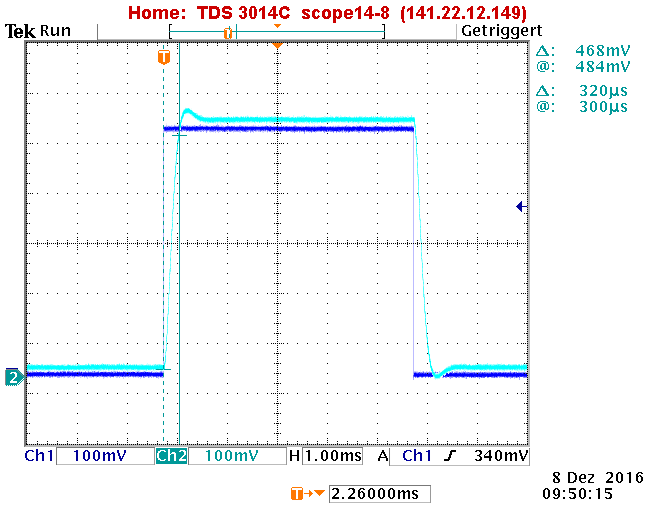
\includegraphics[width=0.60\linewidth]{Bilder/ImLabor/Sprungantwort_5_7_Butter_Einschwingzeit}
	\caption{Sprungantwort Butterworth: Messung der Einschwingzeit}
	\label{fig:Sprungantwort_5_7_Butter_Einschwingzeit}
\end{figure}

\begin{figure}[h]
	\centering
	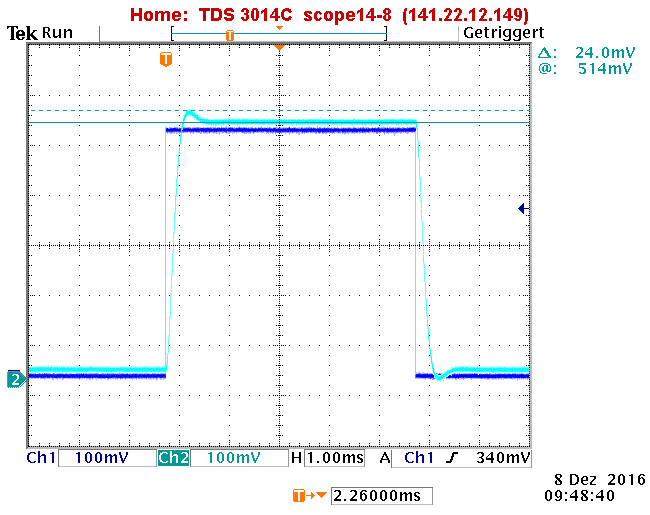
\includegraphics[width=0.60\linewidth]{Bilder/ImLabor/Sprungantwort_5_6_Butter_Ueberschwinger}
	\caption{Sprungantwort Butterworth: Messung des Überschwingers}
	\label{fig:Sprungantwort_5_6_Butter_Ueberschwinger}
\end{figure}

\newpage

\subsubsection{Tschebyscheff}

\begin{figure}[h]
	\centering
	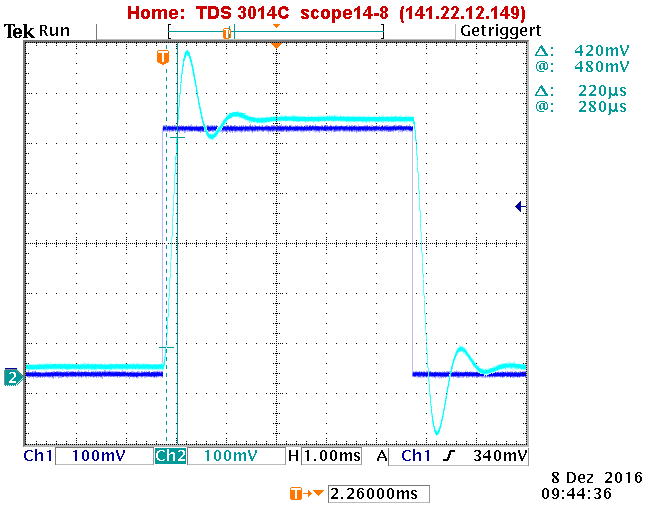
\includegraphics[width=0.60\linewidth]{Bilder/ImLabor/Sprungantwort_5_3_Tscheby_Anstiegszeit}
	\caption{Sprungantwort Tschebyscheff: Messung der Anstiegszeit}
	\label{fig:Sprungantwort_5_3_Tscheby_Anstiegszeit_Anhang}
\end{figure}

\begin{figure}[h]
	\centering
	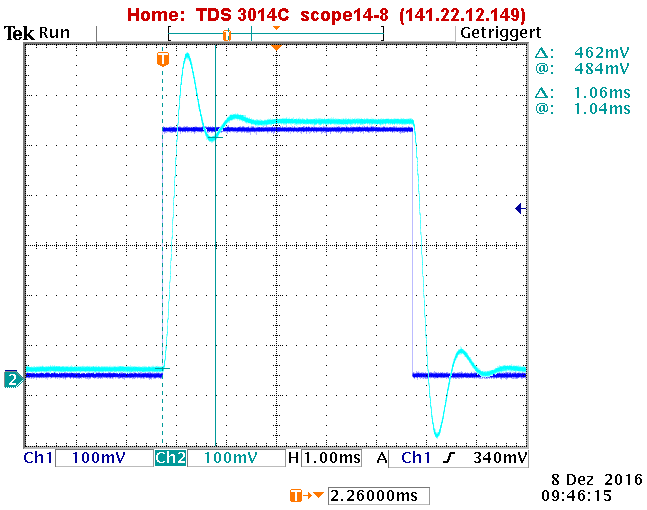
\includegraphics[width=0.60\linewidth]{Bilder/ImLabor/Sprungantwort_5_4_Tscheby_Einschwingzeit}
	\caption{Sprungantwort Tschebyscheff: Messung der Einschwingzeit}
	\label{fig:Sprungantwort_5_4_Tscheby_Einschwingzeit}
\end{figure}

\begin{figure}[h]
\centering
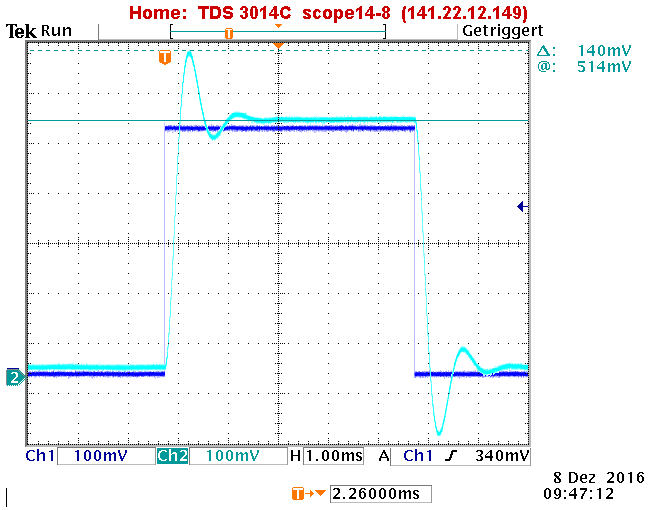
\includegraphics[width=0.60\linewidth]{Bilder/ImLabor/Sprungantwort_5_5_Tscheby_Ueberschwinger}
\caption{Sprungantwort Tschebyscheff: Messung des Überschwingers}
\label{fig:Sprungantwort_5_5_Tscheby_Ueberschwinger}
\end{figure}

\newpage

\subsubsection{Bessel}

\begin{figure}[h]
\centering
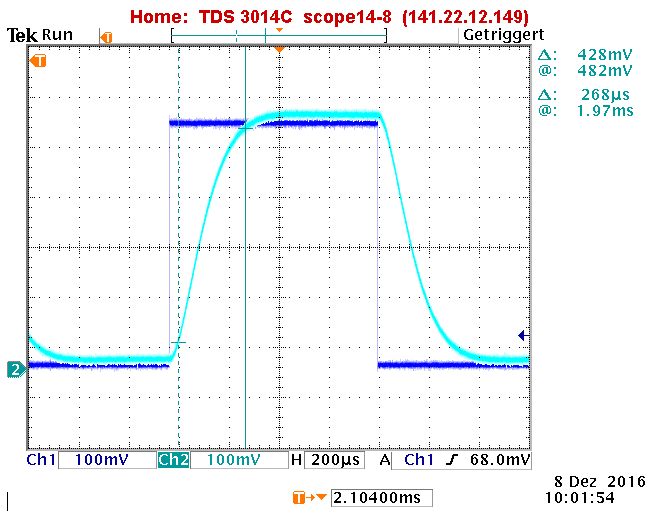
\includegraphics[width=0.60\linewidth]{Bilder/ImLabor/Sprungantwort_5_1_Bessel_Anstiegszeit}
\caption{Sprungantwort Bessel: Messung der Anstiegszeit}
\label{fig:Sprungantwort_5_1_Bessel_Anstiegszeit_Anhang}
\end{figure}

\begin{figure}[h]
\centering
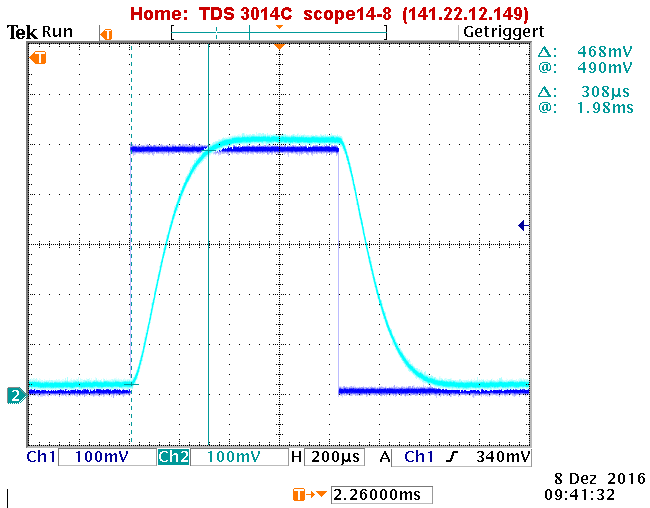
\includegraphics[width=0.60\linewidth]{Bilder/ImLabor/Sprungantwort_5_2_Bessel_Einschwingzeit}
\caption{Sprungantwort Bessel: Messung der Einschwingzeit}
\label{fig:Sprungantwort_5_2_Bessel_Einschwingzeit}
\end{figure}












\noindent \textbf{Unter folgenden Link kann eine \glqq Education\grqq~ Version von PSPice heruntergeladen werden.}
http://www.orcad.com/buy/orcad-educational-program


